\documentclass[../../Main_ManuscritThese.tex]{subfiles}

\subfileGlobal{
\renewcommand{\RootDir}[1]{./Text/Chapter4/#1}
}
\newcommand{\IMSE}{\mathop{IMSE}}

% For cross referencing
\subfileLocal{
\externaldocument{../../Text/Introduction/build/Introduction}
\externaldocument{../../Text/Chapter2/build/Chapter2}
\externaldocument{../../Text/Chapter3/build/Chapter3}
\externaldocument{../../Text/Chapter5/build/Chapter5}
\externaldocument{../../Text/Conclusion/build/Conclusion}
}

%%%%%%%%%%%%%%%%%%%%%%%%%%%%%%%%%%%%%%
%% CHAPTER TITLE
%%%%%%%%%%%%%%%%%%%%%%%%%%%%%%%%%%%%%%

\begin{document}

% \subfileLocal{\setcounter{chapter}{2}}
\specialchapter{Adaptative design enrichment for calibration using Gaussian Processes}
\label{chap:adaptative_design_gp}
\minitoc
\newpage
\subfileLocal{\pagestyle{contentStyle}}
%%%%%%%%%%%%%%%%%%%%%%%%%%%%%%%%%%%%%%%%%%%%%%%%%%%%%%%
%%%%%%%%%%%%%%%%%%%%%%%%%%%%%%%%%%%%%%%%%%%%%%%%%%%%%%%


%%%%%%%%%%%%%%%%%%%%%%%%%%%%%%%%%%%%%%%%%%%%%%%%%%%%%%
%%% 				SECTION 0 : Introduction	   %%%



\section{GP, RR-based family of estimators}
\subsection{Random processes and Gaussian Process Regression}
Let us assume that we have a map $f$ from a $p$ dimensional space to $\mathbb{R}$:
\begin{align}
  \begin{array}{rrcl}
    f: & \mathbb{X} \subset \mathbb{R}^p& \longrightarrow & \mathbb{R} \\
       & x & \longmapsto & f(x)
  \end{array}
\end{align}
This function is assumed to have been evaluated on a design of $n$ points, $\mathcal{X} \subset \mathbb{X}^n$. 
We wish to have a probabilistic modelling of this function
We introduce random processes as way to have a prior distribution on function
This uncertainty on $f$ is modelled as a random process:
\begin{equation}
  \begin{array}{rcl}
    Z: \mathbb{X} \times \Omega& \longrightarrow & \mathbb{R} \\
    (x,\omega) & \longmapsto & Z(x,\omega)
  \end{array}
\end{equation}
The $\omega$ variable will be omitted next.
\subsection{Linear Estimation}
\label{sec:linear_estimation}
A linear estimation $\hat{Z}$ of $f$ at an unobserved point $x\notin \mathcal{X}$ can be written as
\begin{equation}
  \label{eq:lin_est}
  \hat{Z}(x) =
  \begin{bmatrix}
    w_1 \dots w_n
    \end{bmatrix}
    \begin{bmatrix}
      f(x_1) \\ \vdots \\ f(x_n)
    \end{bmatrix} = \mathbf{W}^Tf(\mathcal{X}) = \sum_{i=1}^n w_i(x) f(x_i)
\end{equation}
Using those kriging weights $\mathbf{W}$, a few additional conditions must be added, in order to obtain the Best Linear Unbiased Estimator:
\begin{itemize}
\item Non-biased estimation: $\Ex[\hat{Z}(x) - Z(x)]=0$
\item Minimal variance: $\min~\Ex[(\hat{Z}(x) - Z(x))^2]$
\end{itemize}
Translating using~\cref{eq:lin_est}:
\begin{equation}
  \Ex[\hat{Z}(x) - Z(x)]=0 \iff m(\sum_{i=1}^n w_i(x)-1) = 0 \iff \sum_{i=1}^n w_i(x) = 1 \iff \mathbf{1}^T \mathbf{W} = 1
\end{equation}
For the minimum of variance, we introduce the augmented random vectors $\mathbf{Z}_n(x) = [Z(x_1),\dots Z(x_n), Z(x)]$ and $\mathbf{Z}_n = [Z(x_1),\dots Z(x_n)]$, and
the variance can be expressed as:
\begin{align}
  \Ex[(\hat{Z}(x) - Z(x))^2] &= \Cov\left[[\mathbf{W}^T, -1] \cdot \mathbf{Z}_n(x) \right] \\
                             &= [\mathbf{W}^T, -1] \Cov\left[\mathbf{Z}_n(x) \right] [\mathbf{W}^T, -1]^T
\end{align}
In addition, we have
\begin{equation}
  \Cov\left[\mathbf{Z}_n(x) \right] =
  \begin{bmatrix}
    \Cov\left[ \mathbf{Z}_n^T\right]
    & \Cov\left[\mathbf{Z}_n^T, Z(x) \right]
  \\
  \Cov\left[\mathbf{Z}_n^T, Z(x) \right]^T & \Var\left[Z(x)\right]
  \end{bmatrix}
\end{equation}
Once expanded, the kriging weights solve then the following optimisation problem:
\begin{align}
  \min_{\mathbf{W}} ~&~\mathbf{W}^T \Cov\left[\mathbf{Z}_n\right] \mathbf{W}+ \Var\left[Z(x)\right] \\ &-\Cov\left[\mathbf{Z}_n^T, Z(x) \right]^T \mathbf{W}- \mathbf{W}^T\Cov\left[\mathbf{Z}_n^T, Z(x) \right] \\ 
  \text{s.t. }&  \mathbf{1}^T\mathbf{W} = 1
\end{align}
This leads to
\begin{align}
  \begin{bmatrix}
    \mathbf{W} \\ m
  \end{bmatrix}
  &=
  \begin{bmatrix}
    \Cov\left[\mathbf{Z}_n\right] & \mathbf{1} \\
  \mathbf{1}^T & 0
\end{bmatrix}^{-1}
                 \begin{bmatrix}
                  \Cov\left[\mathbf{Z}_n^T, Z(x) \right]^T \\ 1 
\end{bmatrix}
  \\ &=
    \begin{bmatrix}
      C(x_1, x_1) & \cdots & C(x_1, x_n) & 1 \\
      C(x_2, x_1) & \cdots & C(x_2, x_n) & 1 \\
      \vdots & \ddots & \vdots & \vdots \\
      C(x_n, x_1) & \cdots & C(x_n, x_n)& 1 \\
      1 & \cdots & 1 & 0
    \end{bmatrix}^{-1}
                       \begin{bmatrix}
                         C(x_1, x) \\
                         C(x_2, x) \\
                         \vdots \\
                         C(x_n, x) \\
                         1
                       \end{bmatrix}
\end{align}
and
\begin{equation}
  \hat{Z}(x) =
      \begin{bmatrix}
      C(x_1, x) &
      C(x_2, x) &
      \dots &
      C(x_n, x)
      \end{bmatrix}
      \left(\begin{bmatrix} C(x_1, x_1) & \cdots & C(x_1, x_n)\\
      C(x_2, x_1) & \cdots & C(x_2, x_n) \\
      \vdots & \ddots & \vdots  \\
      C(x_n, x_1) & \cdots & C(x_n, x_n) \\
    \end{bmatrix}^{-1}\right)^T
  \begin{bmatrix}
    f(x_1) \\ f(x_2) \\ \vdots \\ f(x_n)
  \end{bmatrix}
\end{equation}
\subsection{Covariance functions}
\todo{to write}
\label{sec:cov_fun}
\begin{itemize}
\item Desired properties
  \begin{itemize}
  \item isotropy (?)
  \item stationarity
  \item semi-definite positiveness
  \end{itemize}
\item parametric models of covariance
\item examples
\item usual hyperparameters estimation
\end{itemize}

\subsection{Enrichment strategies for Gaussian Processes}
\label{sec:enrichment_strategies}
For a unknown function $f$, a GP is initally constructed based on a design $\mathcal{X} = \left\{\left(x_1,f(x_1)\right), \dots, \left(x_n, f(x_n)\right)\right\}$, that consists of $n$ points of $\Xspace$, and their corresponding evaluations. This GP is denoted $Y \mid \mathcal{X}$ and:
\begin{equation}
  \label{eq:YgivenXGP}
  Y\mid \mathcal{X} \sim \mathcal{N}(m_{Y\mid\mathcal{X}}(x),\sigma^2_{Y\mid\mathcal{X}}(x))
\end{equation}
The main idea behind Stepwise Uncertainty Reduction is to define a criterion, say $\kappa_n$, that measures in a way the uncertainty upon a certain objective associated with the GP and $f$, and to maximize this criterion, in order to select the next point:
\begin{equation}
  x_{n+1} = \argmax_{x\in\Xspace} \kappa_n(x) = \argmax_{x\in\Xspace} \kappa(x; Y \mid \mathcal{X})
\end{equation}
This new point is then evaluated by $f$, and the pair is added to the design: $\mathcal{X} \gets \mathcal{X} \cup \{(x_{n+1}, f(x_{n+1})\}$.
\subsubsection{Exploration based criteria}

We are going to introduce common criteria of enrichment, that aim at exploring the input space $\Xspace$

\paragraph{Maximum variance}
A measure of uncertainty on the GP is $\max_{x\in\Xspace} \sigma_{Y \mid \mathcal{X}}^2(x)$, the maximum value of the prediction variance on the space.
A simple criterion is to select and evaluate the point corresponding to this maximum of variance:
\begin{equation}
  x_{n+1} = \argmax_{x\in \Xspace} \kappa_n(x) = \argmax_{x \in \Xspace} \sigma^2_{Y \mid \mathcal{X}}(x)
\end{equation}
This criterion by its simplicity is easy to implement, as the prediction variance is cheap to compute given a GP, and does not depend directly on the evaluations of the function $f(x_i)$, uniquely on the distance between the inputs points and the covariance parameters.

\paragraph{Integrated Mean Square Error}
\cite{sacks_designs_1989}
The prediction variance is directly given by $\sigma^2_{Y\mid \mathcal{X}}$ and represents the uncertainty on the Gaussian regression. To summarize this uncertainty on the whole space $\mathcal{X}$, we define the Integrated Mean Square Error (IMSE) as
\begin{equation}
  \IMSE(Y \mid \mathcal{X}) = \int_{\Xspace} \sigma_{Y\mid\mathcal{X}}^2(x)\,\mathrm{d}x
\end{equation}
For practical reasons, we can consider to integrate the MSE only on a subset $\mathfrak{X}\subset \mathcal{X}$ that yields
\begin{equation}
  \IMSE\left(Y,\mathfrak{X} \mid \mathcal{X} \right) = \int_{\mathcal{X}} \sigma^2_{Y\mid \mathcal{X}}(x)  \mathbbm{1}_{\{x \in \mathfrak{X}\}}(x)\,\mathrm{d}x = \int_{\mathfrak{X}} \sigma^2_{Y\mid \mathcal{X}}(x)\,\mathrm{d}x
\end{equation}

Unfortunately, exact evaluation of this integral is impossible, so it needs to be approximated using numerical integration, such as Monte-carlo or quadrature rules:
\begin{equation}
  \IMSE(Y,\mathfrak{X} \mid \mathcal{X}) \approx \sum_{i=1}^{n_{\mathrm{quad}}} w_i \sigma_{Y\mid\mathcal{X}}(x_i)
\end{equation}

For a given $x\in \Xspace$ and an outcome $y\in\Yspace$, the augmented design is defined as the experimental design, $\mathcal{X} \cup \left\{(x, y)\right\}$, and the IMSE of the augmented design is $\IMSE\left(Y \mid \mathcal{X} \cup \left\{(x, y)\right\} \right)$. Before the actual experiment though, $y$ is unknown, but we can model it by its distribution given by the GP (per~\cref{eq:YgivenXGP}). So for a given candidate $x$, the mean prediction error we will get when evaluating $x$ is given by
\begin{equation}
  \label{eq:IMSE_augmented}
  \Ex_{Y(x)}\Big[\IMSE\big(Y \mid \mathcal{X} \cup \left\{(x, Y(x))\right\} \big)\Big]
\end{equation}
where the expectation is to be taken with respect to different realisations of $Y(x)$. As each scenario requires to fit a GP, and to compute the IMSE, a precise evaluation is quite expensive. A strategy ffound for instance in~\cite{villemonteix_informational_2006} is to take $M$ possible outcomes for $Y(x)$, corresponding to evenly spaced quantiles of the its distribution.
It is maybe important to note that the hyperparameters of the GP should not be reevaluated when augmenting the design, in order to get comparable values for the IMSE.

To enrich the design with the best point, that reduces the most the prediction error, a simple $1$-step strategy is to minimize the expectation of~\cref{eq:IMSE_augmented}.
\begin{equation}
  x_{n+1} = \argmin_{x\in \Xspace}\Ex_{Y(x)}\Big[\IMSE\big(Y \mid \mathcal{X} \cup \left\{(x, Y(x))\right\} \big)\Big]
\end{equation}



\subsubsection{Contour and volume estimation}
Let us start by introducing diverse tools based around Vorob'ev expectation of closed sets (\cite{el_amri_analyse_2019},~\cite{heinrich_level_2012}). 


Let us consider $A$, a random closed set, such that its realizations are subsets of $\Xspace$, and $p$ is its coverage probability, that is
\begin{equation}
  p(\theta) = \Prob\left[\theta\in A\right], \theta\in\Xspace
\end{equation}
For $\eta \in [0, 1]$, we define the $\eta$-level set of $p$,
\begin{equation}
  Q_{\eta} = \{x\in\Xspace \mid p(x) \geq \eta \}
\end{equation}
It may seem trivial, but let us still note that those sets are decreasing:
\begin{equation}
  0\leq \eta \leq \xi \leq 1 \implies Q_{\xi} \subseteq Q_{\eta}
\end{equation}

Let $\mu$ be a Borel $\sigma$-finite measure on $\Xspace$. We define Vorob'ev expectation, as the $\eta^*$-level set of $A$ verifying
\begin{equation}
  \forall \beta < \eta^* \quad \mu(Q_{\beta}) \leq \Ex[\mu(A)] \leq \mu(Q_{\eta^*})
\end{equation}
that is the level set of $p$, that has the volume of the mean of the volume of the random set $A$.

\subsubsection{Margin of uncertainty}
\label{sec:margin_of_uncertainty}
Using the quantiles of this level set, we can construct the $\eta$-margin of uncertainty, as~\cite{dubourg_reliability-based_2011}.
Setting the classical level $\eta=0.05$ for instance, $Q_{1-\frac{\eta}{2}}=Q_{0.975}$ is the set of points whose probability of coverage is higher than $0.975$, while $Q_{\frac{\eta}{2}}=Q_{0.025}$ is the set of points whose probability of coverage is higher than $0.025$. Obviously, $Q_{1-\frac{\eta}{2}} \subset Q_{\frac{\eta}{2}}$. The complement of $Q_{\frac{\eta}{2}}$ in $\Xspace$, denoted by $Q_{\frac{\eta}{2}}^C$ is the set of points whose probability of coverage is lower than $0.025$. The $\eta$-margin of uncertainty $\mathbb{M}_{\eta}$ is defined as the sets of points whose coverage probability is between $0.025$ and $0.975$.
\begin{equation*}
  \mathbb{M}_{\eta} = \left(Q_{1-\frac{\eta}{2}} \cup Q^C_{\frac{\eta}{2}} \right)^C = Q_{1-\frac{\eta}{2}}^C \cap Q_{\frac{\eta}{2}} = Q_{\frac{\eta}{2}} \setminus Q_{1-\frac{\eta}{2}}
\end{equation*}


% \subsubsection{Contour and volume estimation}

% Let $Y$ be a random process over $\Xspace$, and let us follow what has been done in~\cite{bect_sequential_2012}.
% Let $\mathfrak{F} \subset \mathbb{R}$ be a region of failure: $f^{-1}(\mathfrak{F})$



\subsection{Estimation of relative-regret quantities}
\subsubsection{GP of the penalized cost function $\Delta_{\alpha}$}
\label{ssec:gp_delta_alpha}
We assume that we constructed a GP on $J$ on the joint space $\Kspace \times \Uspace$, based on a design of $n$ points $\mathcal{X} = \left\{(\kk^{(1)},\uu^{(1)}),\dots,(\kk^{(n)},\uu^{(n)}) \right\}$, denoted as $(\kk,\uu)\mapsto Y(\kk,\uu)$.

As a GP, $Y$ is described by its mean function $m_{Y}$ and its covariance function $C(\cdot, \cdot)$, while $\sigma^2_Y(\kk,\uu) = C((\kk,\uu), (\kk,\uu))$
\begin{equation}
  Y(\kk,\uu) \sim \mathcal{N}\left(m_{Y}(\kk,\uu), \sigma^2_Y(\kk,\uu) \right)
\end{equation}
Let us consider now the conditional minimiser:
\begin{align}
  J^*(\uu) = J(\kk^*(\uu),\uu) = \min_{\kk\in\Kspace} J(\kk,\uu)
\end{align}

Analogous to $J$ and $J^*$, we define $Y^*$ as
\begin{equation}
  Y^*(\uu) \sim \mathcal{N}\left(m^*_Y(\uu), \sigma^{2,*}_Y(\uu)\right)
\end{equation}
where
\begin{align}
  m^*_Y(\uu) = \min_{\kk\in\Kspace} m_Y(\kk,\uu) = m_Y(\kk^*(\uu)) \\
  \sigma^{2,*}_Y(\uu) = \sigma^{2,*}_Y(\kk^*(\uu)) 
\end{align}
The surrogate conditional minimiser is used in~\cite{ginsbourger_bayesian_2014} for instance, but other choices could be considered, such as $m_Y(\kk^*(\uu)) - \beta \sigma^{2,*}_Y(\kk^*(\uu))$. This choice for instance would lead to be more ``optimistic'' in the estimation of the minimum (i.e.\ a lower minimum), and in turn, would have a tendency to overestimate the estimated value of $\alpha$.

The $\alpha$-relaxed difference defined as  $\Delta_{\alpha} = Y - \alpha Y^*$ is a linear combination of correlated Gaussian processes. Its distribution is Gaussian and can be derived by first considering the joint distribution of $Y(\kk,\uu)$ and $Y^*(\uu) = Y(\kk^*(\uu), \uu)$:
\begin{equation}
  \begin{bmatrix}
    Y(\kk,\uu) \\
    Y^*(\uu)
  \end{bmatrix}
  \sim \mathcal{N}\left(
    \begin{bmatrix}
      m_Y(\kk,\uu) \\
      m_Y^*(\uu)
    \end{bmatrix}
    ;\,
    \begin{bmatrix}
      C\left((\kk,\uu),(\kk,\uu)\right) & C\left((\kk,\uu),(\kk^*(\uu),\uu)\right) \\
      C\left((\kk,\uu),(\kk^*(\uu),\uu)\right) & C\left((\kk^*(\uu),\uu),(\kk^*(\uu),\uu)\right)
    \end{bmatrix}
\right)
\end{equation}
Multiplying by the matrix $\begin{bmatrix}1 & -\alpha \end{bmatrix}$ yields

\begin{align}
  \Delta_{\alpha}(\kk,\uu) &\sim \mathcal{N}\left(m_{\Delta}(\kk,\uu); \sigma^2_{\Delta}(\kk,\uu)\right)  \label{eq:delta_GP}\\
  m_{\Delta}(\kk,\uu) &= m_Y(\kk,\uu) - \alpha m_Y^*(\uu) \label{eq:mu_delta_GP}\\
  \sigma^2_{\Delta}(\kk,\uu) &= \sigma_Y^2(\kk,\uu) + \alpha^2 \sigma_{Y^*}^2(\kk,\uu) - 2\alpha C\left((\kk,\uu),(\kk^*(\uu),\uu)\right) \label{eq:variance_delta_GP}
\end{align}


Decomposing the variance $\sigma^2_{\Delta}$ in~\cref{eq:variance_delta_GP}, 3 sources of uncertainty arise:
\begin{itemize}
\item $\sigma^2_{Y}$ is the prediction variance of the GP on $J$, that is directly reduced when additional points are evaluated
\item $\sigma^2_{Y^*}$ is the variance of the predicted value of the minimizer.
  
\item Assuming a stationary form of the covariance, the third term is directly dependent on the distance between $\kk$ and $\kk^*(\uu)$. As the covariance term can be written $C((\kk,\uu), (\kk',\uu')) = s \prod_{i\in\mathcal{I}_{\kk}}\rho_{\theta_i}(\|k_i - k'_i\|) \prod_{j\in\mathcal{I}_{\uu}} \rho_{\theta_j}(\|u_j - u'_j\|)$, substituting $\kk^*(\uu)$ for $\kk^\prime$ gives
\begin{align}
  C\left((\kk,\uu),(\kk^*(\uu),\uu)\right) &= s \prod_{i\in\mathcal{I}_{\kk}}\rho_{\theta_i}(\|k_i - k^*_i(\uu)\|)\prod_{j\in\mathcal{I}_{\uu}} \rho_{\theta_j}(0) \\
  &=s \prod_{i\in\mathcal{I}_{\kk}}\rho_{\theta_i}(\|k_i - k^*_i(\uu)\|)
\end{align}
\end{itemize}
This decomposition highlights the fact that the uncertainty measured at a point $(\kk, \uu)$ using $\sigma_{\Delta}^2$ will not be reduced completely by evaluating the function at this point, as only the prediction variance $\sigma_Y^2$ will be significantly affected in general. In this case, reducing the uncertainty on a slice of constant $\kk$ (candidate) will not result necessarily in an evaluation on this slice.


\subsubsection{Approximation of the targeted probability using GP}

% We are going now to use a different notation for the probabilities, taken with respect to the GP: $\ProbGP$, to represent the uncertainty encompassed by the GP:
% \begin{equation}
%   \ProbGP[A] = \int_{A} \, \mathrm{d}\ProbGP(\xi)
% \end{equation}
  
\paragraph{Through the probability of coverage}


For a given $\kk\in\Kspace$, the coverage probability of the $\alpha$-acceptable region, i.e.\ the probability for $\kk$ to be $\alpha$-acceptable is
\begin{align}
  \Gamma_{\alpha}(\kk) &= \Prob_{U}\left[J(\kk,\UU) \leq \alpha J^*(\UU)\right] \\
                              & =\Ex_{U}\left[\mathbbm{1}_{J(\kk,\UU) \leq \alpha J^*(\UU)}\right]
\end{align}
As $J$ is not known perfectly, it devolves into a classification problem
This classification problem can be approached with a plug-in approach in~\cref{eq:plugin_indicator}, or a probabilistic one in~\cref{eq:prob_indicator}:
\begin{align}
  \mathbbm{1}_{J(\kk,\uu) \leq \alpha J^*(\uu)} &\approx   \mathbbm{1}_{m_Y(\kk,\uu) \leq \alpha m_Y^*(\uu)} \label{eq:plugin_indicator} \\
  \mathbbm{1}_{J(\kk,\uu) \leq \alpha J^*(\uu)} &\approx   \ProbGP\left[ \Delta_{\alpha}(\kk,\uu) \leq 0 \right] = \pi_{\alpha}(\kk,\uu) \label{eq:prob_indicator}
\end{align}
Using the GPs, for a given $\kk$, $\alpha$ and $\uu$, the probability for our metamodel to verify the inequality is given by
Based on those two approximation, we can define different estimations of $\Gamma$
\begin{align}
  \hat{\Gamma}_{\alpha, n}(\kk) &= \Prob_U\left[m_Y(\kk,\uu) \leq \alpha m_Y^*(\uu) \right] \tag{plug-in} \\
  \hat{\Gamma}_{\alpha, n}(\kk) &= \Ex_U\left[ \ProbGP\left[ \Delta_{\alpha}(\kk,\uu) \leq 0\right]\right]  = \Ex_U\left[\pi_{\alpha}(\kk,\uu)\right]\tag{Probabilistic approx} \\
\end{align}

The probability of coverage for the set $\{Y - \alpha Y^*\leq 0\}$ is $\pi_{\alpha}$, and can be computed using the CDF of the standard normal distribution $\Phi$, because $\Delta_{\alpha}$ is a GP, as defined in~\cref{eq:delta_GP,eq:mu_delta_GP,eq:variance_delta_GP}
\begin{equation}
  \pi_{\alpha}(\kk,\uu) = \Phi\left(-\frac{m_{\Delta_\alpha}(\kk,\uu)}{\sigma_{\Delta_\alpha}(\kk,\uu)}\right)
\end{equation}
Finally, averaging over $\uu$ yields
\begin{equation}
  \hat{\Gamma}_{\alpha,n}(\kk) = \Ex_U\left[\pi_{\alpha}(\kk,\uu)\right]=\int_{\Uspace}\pi_{\alpha}(\kk,\uu)p(\uu) \,\mathrm{d}\uu = \int_{\Uspace}\Phi\left(-\frac{m_{\Delta_\alpha}(\kk,\uu)}{\sigma_{\Delta_\alpha}(\kk,\uu)}\right)p(\uu) \,\mathrm{d}\uu
\end{equation}

The estimation of $\Gamma$ is then maximised with respect to $\kk$ to get the candidate probability
\begin{equation}
\max_{\kk\in\Kspace}  \hat{\Gamma}_{\alpha,n}(\kk) 
\end{equation}
By tweaking the value of $\alpha$, we can get the estimate $\hat{\Gamma}$ to have its maximum equal to the targeted probability. 
As pointed out earlier the estimation of $\alpha_p$ depends on the estimation of $\hat{\Gamma}$.
\paragraph{$\alpha$ through quantiles}
Instead of maximizing for each $\alpha$ the estimated $\hat{\Gamma}$, we are now going to derive an approach based on the quantiles:
Let $Y(\kk, \uu) \sim \mathcal{N}(m_Y(\kk,\uu), \sigma^2_{Y}(\kk, \uu))$ be the GP fitted using $\mathcal{X}$. A realisation $y\sim Y$ is then a function from $\Kspace \times \Uspace$ to $\mathbb{R}^{+}_*$.
Again, the plug-in approach is to compute the ratio $m_Y(\kk, \uu) / m^*_Y(\uu)$ on a large grid for $\uu$ and for each $\kk$, look for the quantile of order $p$ with respect to $\UU$
\begin{equation}
  \alpha_{m_{Y}}(\kk) = Q_{U}\left(p;~\frac{m_Y(\kk, \UU)}{m^*_Y(\UU)}\right)
\end{equation}
the estimation of the relaxation value $\hat{\alpha}_p$ is then the minimal value of the quantiles with respect to $\kk$:
\begin{equation}
    \label{eq:def_plugin_alpha}
  \hat{\alpha}^{\mathrm{PI}}_p = \min_{\kk \in \Kspace} Q_U\left(p;~\frac{m_Y(\kk, \UU)}{m^*_Y(\UU)}\right)  \tag{plug-in}
\end{equation}
Moreover, as we can sample quite easily from the GP, we can have an idea of the uncertainty in the estimation of $\hat{\alpha}_p$.
Let us say that we sampled $N$ function from $Y$, namely $y^{(i)}$ for $1 \leq i \leq N$. For each of these samples, we can get $\alpha_{y^{(i)}}(\kk)$, shortened as $\alpha^{(i)}(\kk)$. Using Monte-Carlo, we can approximate the usual moments for $\alpha$.

\begin{equation}
 \Ex_{Y}\left[\alpha_{Y}(\kk) \right] \approx \frac{1}{N} \sum_{i=1}^N \alpha^{(i)}(\kk) = \alpha^{\mathrm{MC}}(\kk)
\end{equation}

and finally,
\begin{equation}
  \hat{\alpha}_p^{\mathrm{MC}} = \min_{\kk \in \Kspace} \alpha^{\mathrm{MC}}(\kk)
\end{equation}


\paragraph{Iterative procedure}
The general
\cref{ssec:gp_delta_alpha}
\begin{itemize}
\item Find a measure of uncertainty that depends as a function of $\kk \times \Uspace$.
\item Find the point that reduces the most the uncertainty on this slice
\item Update
\end{itemize}

At the step $n$:
\begin{itemize}
\item First, using the GP, $\alpha_p$ is estimated using Monte-carlo and samples from the GP, giving $\hat{\alpha}_{n,.99}$
\item We choose the candidate $\kk_{\mathrm{candidate}}$ as the minimizer of the sampled quantiles: $\kk_{\mathrm{candidate}} = \argmin_{\kk} \alpha^{\mathrm{MC}}(\kk)$.
\item We optimize the wIMSE, defined as $\IMSE(Y_n \mid \mathcal{X}, \{\kk_{\mathrm{candidate}}\}\times \Uspace )$ to get the next point to sample
\end{itemize}
On Figure~\cref{fig:alpha_MC} is shown the procedure applied on BHs, based on a initial design of $30$ points. The wIMSE is computed by sampling a $50$-point LHS on $\{\kk_{\mathrm{candidate}} \times \Uspace\}$.
The estimation using Monte-carlo seems to show convergence towards the true value, while the plug-in approach does not evolve much with the iterations
\begin{figure}[!h]
  \centering
  %% Creator: Matplotlib, PGF backend
%%
%% To include the figure in your LaTeX document, write
%%   \input{<filename>.pgf}
%%
%% Make sure the required packages are loaded in your preamble
%%   \usepackage{pgf}
%%
%% Figures using additional raster images can only be included by \input if
%% they are in the same directory as the main LaTeX file. For loading figures
%% from other directories you can use the `import` package
%%   \usepackage{import}
%% and then include the figures with
%%   \import{<path to file>}{<filename>.pgf}
%%
%% Matplotlib used the following preamble
%%   \usepackage{fontspec}
%%   \setmainfont{DejaVuSans.ttf}[Path=/home/victor/miniconda3/lib/python3.7/site-packages/matplotlib/mpl-data/fonts/ttf/]
%%   \setsansfont{LiberationSans-Regular.ttf}[Path=/usr/share/fonts/truetype/liberation/]
%%   \setmonofont{DejaVuSansMono.ttf}[Path=/home/victor/miniconda3/lib/python3.7/site-packages/matplotlib/mpl-data/fonts/ttf/]
%%
\begingroup%
\makeatletter%
\begin{pgfpicture}%
\pgfpathrectangle{\pgfpointorigin}{\pgfqpoint{5.748032in}{3.552479in}}%
\pgfusepath{use as bounding box, clip}%
\begin{pgfscope}%
\pgfsetbuttcap%
\pgfsetmiterjoin%
\definecolor{currentfill}{rgb}{1.000000,1.000000,1.000000}%
\pgfsetfillcolor{currentfill}%
\pgfsetlinewidth{0.000000pt}%
\definecolor{currentstroke}{rgb}{1.000000,1.000000,1.000000}%
\pgfsetstrokecolor{currentstroke}%
\pgfsetdash{}{0pt}%
\pgfpathmoveto{\pgfqpoint{0.000000in}{0.000000in}}%
\pgfpathlineto{\pgfqpoint{5.748032in}{0.000000in}}%
\pgfpathlineto{\pgfqpoint{5.748032in}{3.552479in}}%
\pgfpathlineto{\pgfqpoint{0.000000in}{3.552479in}}%
\pgfpathclose%
\pgfusepath{fill}%
\end{pgfscope}%
\begin{pgfscope}%
\pgfsetbuttcap%
\pgfsetmiterjoin%
\definecolor{currentfill}{rgb}{0.917647,0.917647,0.949020}%
\pgfsetfillcolor{currentfill}%
\pgfsetlinewidth{0.000000pt}%
\definecolor{currentstroke}{rgb}{0.000000,0.000000,0.000000}%
\pgfsetstrokecolor{currentstroke}%
\pgfsetstrokeopacity{0.000000}%
\pgfsetdash{}{0pt}%
\pgfpathmoveto{\pgfqpoint{0.424692in}{2.286284in}}%
\pgfpathlineto{\pgfqpoint{5.598032in}{2.286284in}}%
\pgfpathlineto{\pgfqpoint{5.598032in}{3.192518in}}%
\pgfpathlineto{\pgfqpoint{0.424692in}{3.192518in}}%
\pgfpathclose%
\pgfusepath{fill}%
\end{pgfscope}%
\begin{pgfscope}%
\pgfpathrectangle{\pgfqpoint{0.424692in}{2.286284in}}{\pgfqpoint{5.173340in}{0.906234in}}%
\pgfusepath{clip}%
\pgfsetroundcap%
\pgfsetroundjoin%
\pgfsetlinewidth{1.003750pt}%
\definecolor{currentstroke}{rgb}{1.000000,1.000000,1.000000}%
\pgfsetstrokecolor{currentstroke}%
\pgfsetdash{}{0pt}%
\pgfpathmoveto{\pgfqpoint{0.659844in}{2.286284in}}%
\pgfpathlineto{\pgfqpoint{0.659844in}{3.192518in}}%
\pgfusepath{stroke}%
\end{pgfscope}%
\begin{pgfscope}%
\definecolor{textcolor}{rgb}{0.150000,0.150000,0.150000}%
\pgfsetstrokecolor{textcolor}%
\pgfsetfillcolor{textcolor}%
\pgftext[x=0.659844in,y=2.189062in,,top]{\color{textcolor}\rmfamily\fontsize{10.000000}{12.000000}\selectfont \(\displaystyle 0\)}%
\end{pgfscope}%
\begin{pgfscope}%
\pgfpathrectangle{\pgfqpoint{0.424692in}{2.286284in}}{\pgfqpoint{5.173340in}{0.906234in}}%
\pgfusepath{clip}%
\pgfsetroundcap%
\pgfsetroundjoin%
\pgfsetlinewidth{1.003750pt}%
\definecolor{currentstroke}{rgb}{1.000000,1.000000,1.000000}%
\pgfsetstrokecolor{currentstroke}%
\pgfsetdash{}{0pt}%
\pgfpathmoveto{\pgfqpoint{1.322243in}{2.286284in}}%
\pgfpathlineto{\pgfqpoint{1.322243in}{3.192518in}}%
\pgfusepath{stroke}%
\end{pgfscope}%
\begin{pgfscope}%
\definecolor{textcolor}{rgb}{0.150000,0.150000,0.150000}%
\pgfsetstrokecolor{textcolor}%
\pgfsetfillcolor{textcolor}%
\pgftext[x=1.322243in,y=2.189062in,,top]{\color{textcolor}\rmfamily\fontsize{10.000000}{12.000000}\selectfont \(\displaystyle 10\)}%
\end{pgfscope}%
\begin{pgfscope}%
\pgfpathrectangle{\pgfqpoint{0.424692in}{2.286284in}}{\pgfqpoint{5.173340in}{0.906234in}}%
\pgfusepath{clip}%
\pgfsetroundcap%
\pgfsetroundjoin%
\pgfsetlinewidth{1.003750pt}%
\definecolor{currentstroke}{rgb}{1.000000,1.000000,1.000000}%
\pgfsetstrokecolor{currentstroke}%
\pgfsetdash{}{0pt}%
\pgfpathmoveto{\pgfqpoint{1.984643in}{2.286284in}}%
\pgfpathlineto{\pgfqpoint{1.984643in}{3.192518in}}%
\pgfusepath{stroke}%
\end{pgfscope}%
\begin{pgfscope}%
\definecolor{textcolor}{rgb}{0.150000,0.150000,0.150000}%
\pgfsetstrokecolor{textcolor}%
\pgfsetfillcolor{textcolor}%
\pgftext[x=1.984643in,y=2.189062in,,top]{\color{textcolor}\rmfamily\fontsize{10.000000}{12.000000}\selectfont \(\displaystyle 20\)}%
\end{pgfscope}%
\begin{pgfscope}%
\pgfpathrectangle{\pgfqpoint{0.424692in}{2.286284in}}{\pgfqpoint{5.173340in}{0.906234in}}%
\pgfusepath{clip}%
\pgfsetroundcap%
\pgfsetroundjoin%
\pgfsetlinewidth{1.003750pt}%
\definecolor{currentstroke}{rgb}{1.000000,1.000000,1.000000}%
\pgfsetstrokecolor{currentstroke}%
\pgfsetdash{}{0pt}%
\pgfpathmoveto{\pgfqpoint{2.647042in}{2.286284in}}%
\pgfpathlineto{\pgfqpoint{2.647042in}{3.192518in}}%
\pgfusepath{stroke}%
\end{pgfscope}%
\begin{pgfscope}%
\definecolor{textcolor}{rgb}{0.150000,0.150000,0.150000}%
\pgfsetstrokecolor{textcolor}%
\pgfsetfillcolor{textcolor}%
\pgftext[x=2.647042in,y=2.189062in,,top]{\color{textcolor}\rmfamily\fontsize{10.000000}{12.000000}\selectfont \(\displaystyle 30\)}%
\end{pgfscope}%
\begin{pgfscope}%
\pgfpathrectangle{\pgfqpoint{0.424692in}{2.286284in}}{\pgfqpoint{5.173340in}{0.906234in}}%
\pgfusepath{clip}%
\pgfsetroundcap%
\pgfsetroundjoin%
\pgfsetlinewidth{1.003750pt}%
\definecolor{currentstroke}{rgb}{1.000000,1.000000,1.000000}%
\pgfsetstrokecolor{currentstroke}%
\pgfsetdash{}{0pt}%
\pgfpathmoveto{\pgfqpoint{3.309442in}{2.286284in}}%
\pgfpathlineto{\pgfqpoint{3.309442in}{3.192518in}}%
\pgfusepath{stroke}%
\end{pgfscope}%
\begin{pgfscope}%
\definecolor{textcolor}{rgb}{0.150000,0.150000,0.150000}%
\pgfsetstrokecolor{textcolor}%
\pgfsetfillcolor{textcolor}%
\pgftext[x=3.309442in,y=2.189062in,,top]{\color{textcolor}\rmfamily\fontsize{10.000000}{12.000000}\selectfont \(\displaystyle 40\)}%
\end{pgfscope}%
\begin{pgfscope}%
\pgfpathrectangle{\pgfqpoint{0.424692in}{2.286284in}}{\pgfqpoint{5.173340in}{0.906234in}}%
\pgfusepath{clip}%
\pgfsetroundcap%
\pgfsetroundjoin%
\pgfsetlinewidth{1.003750pt}%
\definecolor{currentstroke}{rgb}{1.000000,1.000000,1.000000}%
\pgfsetstrokecolor{currentstroke}%
\pgfsetdash{}{0pt}%
\pgfpathmoveto{\pgfqpoint{3.971841in}{2.286284in}}%
\pgfpathlineto{\pgfqpoint{3.971841in}{3.192518in}}%
\pgfusepath{stroke}%
\end{pgfscope}%
\begin{pgfscope}%
\definecolor{textcolor}{rgb}{0.150000,0.150000,0.150000}%
\pgfsetstrokecolor{textcolor}%
\pgfsetfillcolor{textcolor}%
\pgftext[x=3.971841in,y=2.189062in,,top]{\color{textcolor}\rmfamily\fontsize{10.000000}{12.000000}\selectfont \(\displaystyle 50\)}%
\end{pgfscope}%
\begin{pgfscope}%
\pgfpathrectangle{\pgfqpoint{0.424692in}{2.286284in}}{\pgfqpoint{5.173340in}{0.906234in}}%
\pgfusepath{clip}%
\pgfsetroundcap%
\pgfsetroundjoin%
\pgfsetlinewidth{1.003750pt}%
\definecolor{currentstroke}{rgb}{1.000000,1.000000,1.000000}%
\pgfsetstrokecolor{currentstroke}%
\pgfsetdash{}{0pt}%
\pgfpathmoveto{\pgfqpoint{4.634240in}{2.286284in}}%
\pgfpathlineto{\pgfqpoint{4.634240in}{3.192518in}}%
\pgfusepath{stroke}%
\end{pgfscope}%
\begin{pgfscope}%
\definecolor{textcolor}{rgb}{0.150000,0.150000,0.150000}%
\pgfsetstrokecolor{textcolor}%
\pgfsetfillcolor{textcolor}%
\pgftext[x=4.634240in,y=2.189062in,,top]{\color{textcolor}\rmfamily\fontsize{10.000000}{12.000000}\selectfont \(\displaystyle 60\)}%
\end{pgfscope}%
\begin{pgfscope}%
\pgfpathrectangle{\pgfqpoint{0.424692in}{2.286284in}}{\pgfqpoint{5.173340in}{0.906234in}}%
\pgfusepath{clip}%
\pgfsetroundcap%
\pgfsetroundjoin%
\pgfsetlinewidth{1.003750pt}%
\definecolor{currentstroke}{rgb}{1.000000,1.000000,1.000000}%
\pgfsetstrokecolor{currentstroke}%
\pgfsetdash{}{0pt}%
\pgfpathmoveto{\pgfqpoint{5.296640in}{2.286284in}}%
\pgfpathlineto{\pgfqpoint{5.296640in}{3.192518in}}%
\pgfusepath{stroke}%
\end{pgfscope}%
\begin{pgfscope}%
\definecolor{textcolor}{rgb}{0.150000,0.150000,0.150000}%
\pgfsetstrokecolor{textcolor}%
\pgfsetfillcolor{textcolor}%
\pgftext[x=5.296640in,y=2.189062in,,top]{\color{textcolor}\rmfamily\fontsize{10.000000}{12.000000}\selectfont \(\displaystyle 70\)}%
\end{pgfscope}%
\begin{pgfscope}%
\definecolor{textcolor}{rgb}{0.150000,0.150000,0.150000}%
\pgfsetstrokecolor{textcolor}%
\pgfsetfillcolor{textcolor}%
\pgftext[x=3.011362in,y=1.999094in,,top]{\color{textcolor}\rmfamily\fontsize{11.000000}{13.200000}\selectfont Number of iterations}%
\end{pgfscope}%
\begin{pgfscope}%
\pgfpathrectangle{\pgfqpoint{0.424692in}{2.286284in}}{\pgfqpoint{5.173340in}{0.906234in}}%
\pgfusepath{clip}%
\pgfsetroundcap%
\pgfsetroundjoin%
\pgfsetlinewidth{1.003750pt}%
\definecolor{currentstroke}{rgb}{1.000000,1.000000,1.000000}%
\pgfsetstrokecolor{currentstroke}%
\pgfsetdash{}{0pt}%
\pgfpathmoveto{\pgfqpoint{0.424692in}{2.368157in}}%
\pgfpathlineto{\pgfqpoint{5.598032in}{2.368157in}}%
\pgfusepath{stroke}%
\end{pgfscope}%
\begin{pgfscope}%
\definecolor{textcolor}{rgb}{0.150000,0.150000,0.150000}%
\pgfsetstrokecolor{textcolor}%
\pgfsetfillcolor{textcolor}%
\pgftext[x=0.258025in,y=2.315395in,left,base]{\color{textcolor}\rmfamily\fontsize{10.000000}{12.000000}\selectfont \(\displaystyle 2\)}%
\end{pgfscope}%
\begin{pgfscope}%
\pgfpathrectangle{\pgfqpoint{0.424692in}{2.286284in}}{\pgfqpoint{5.173340in}{0.906234in}}%
\pgfusepath{clip}%
\pgfsetroundcap%
\pgfsetroundjoin%
\pgfsetlinewidth{1.003750pt}%
\definecolor{currentstroke}{rgb}{1.000000,1.000000,1.000000}%
\pgfsetstrokecolor{currentstroke}%
\pgfsetdash{}{0pt}%
\pgfpathmoveto{\pgfqpoint{0.424692in}{2.792955in}}%
\pgfpathlineto{\pgfqpoint{5.598032in}{2.792955in}}%
\pgfusepath{stroke}%
\end{pgfscope}%
\begin{pgfscope}%
\definecolor{textcolor}{rgb}{0.150000,0.150000,0.150000}%
\pgfsetstrokecolor{textcolor}%
\pgfsetfillcolor{textcolor}%
\pgftext[x=0.258025in,y=2.740194in,left,base]{\color{textcolor}\rmfamily\fontsize{10.000000}{12.000000}\selectfont \(\displaystyle 3\)}%
\end{pgfscope}%
\begin{pgfscope}%
\pgfpathrectangle{\pgfqpoint{0.424692in}{2.286284in}}{\pgfqpoint{5.173340in}{0.906234in}}%
\pgfusepath{clip}%
\pgfsetroundcap%
\pgfsetroundjoin%
\pgfsetlinewidth{1.756562pt}%
\definecolor{currentstroke}{rgb}{0.298039,0.447059,0.690196}%
\pgfsetstrokecolor{currentstroke}%
\pgfsetdash{}{0pt}%
\pgfpathmoveto{\pgfqpoint{0.659844in}{2.337458in}}%
\pgfpathlineto{\pgfqpoint{0.726084in}{2.337366in}}%
\pgfpathlineto{\pgfqpoint{0.792324in}{2.337458in}}%
\pgfpathlineto{\pgfqpoint{0.858564in}{2.335875in}}%
\pgfpathlineto{\pgfqpoint{0.924804in}{2.334836in}}%
\pgfpathlineto{\pgfqpoint{0.991043in}{2.327477in}}%
\pgfpathlineto{\pgfqpoint{1.057283in}{2.333602in}}%
\pgfpathlineto{\pgfqpoint{1.123523in}{2.341533in}}%
\pgfpathlineto{\pgfqpoint{1.189763in}{2.337632in}}%
\pgfpathlineto{\pgfqpoint{1.256003in}{2.338220in}}%
\pgfpathlineto{\pgfqpoint{1.322243in}{2.333514in}}%
\pgfpathlineto{\pgfqpoint{1.388483in}{2.341137in}}%
\pgfpathlineto{\pgfqpoint{1.454723in}{2.337663in}}%
\pgfpathlineto{\pgfqpoint{1.520963in}{2.341984in}}%
\pgfpathlineto{\pgfqpoint{1.587203in}{2.348486in}}%
\pgfpathlineto{\pgfqpoint{1.653443in}{2.347598in}}%
\pgfpathlineto{\pgfqpoint{1.719683in}{2.348192in}}%
\pgfpathlineto{\pgfqpoint{1.785923in}{2.347395in}}%
\pgfpathlineto{\pgfqpoint{1.852163in}{2.356817in}}%
\pgfpathlineto{\pgfqpoint{1.918403in}{2.355011in}}%
\pgfpathlineto{\pgfqpoint{1.984643in}{2.356278in}}%
\pgfpathlineto{\pgfqpoint{2.050883in}{2.357949in}}%
\pgfpathlineto{\pgfqpoint{2.117123in}{2.357349in}}%
\pgfpathlineto{\pgfqpoint{2.183362in}{2.355626in}}%
\pgfpathlineto{\pgfqpoint{2.249602in}{2.355053in}}%
\pgfpathlineto{\pgfqpoint{2.315842in}{2.352012in}}%
\pgfpathlineto{\pgfqpoint{2.382082in}{2.349480in}}%
\pgfpathlineto{\pgfqpoint{2.448322in}{2.350497in}}%
\pgfpathlineto{\pgfqpoint{2.514562in}{2.349609in}}%
\pgfpathlineto{\pgfqpoint{2.580802in}{2.352787in}}%
\pgfpathlineto{\pgfqpoint{2.647042in}{2.353230in}}%
\pgfpathlineto{\pgfqpoint{2.713282in}{2.351777in}}%
\pgfpathlineto{\pgfqpoint{2.779522in}{2.352070in}}%
\pgfpathlineto{\pgfqpoint{2.845762in}{2.362631in}}%
\pgfpathlineto{\pgfqpoint{2.912002in}{2.361797in}}%
\pgfpathlineto{\pgfqpoint{2.978242in}{2.362795in}}%
\pgfpathlineto{\pgfqpoint{3.044482in}{2.354219in}}%
\pgfpathlineto{\pgfqpoint{3.110722in}{2.354450in}}%
\pgfpathlineto{\pgfqpoint{3.176962in}{2.360279in}}%
\pgfpathlineto{\pgfqpoint{3.243202in}{2.359844in}}%
\pgfpathlineto{\pgfqpoint{3.309442in}{2.359035in}}%
\pgfpathlineto{\pgfqpoint{3.375682in}{2.359054in}}%
\pgfpathlineto{\pgfqpoint{3.441921in}{2.362684in}}%
\pgfpathlineto{\pgfqpoint{3.508161in}{2.362010in}}%
\pgfpathlineto{\pgfqpoint{3.574401in}{2.362742in}}%
\pgfpathlineto{\pgfqpoint{3.640641in}{2.362920in}}%
\pgfpathlineto{\pgfqpoint{3.706881in}{2.362866in}}%
\pgfpathlineto{\pgfqpoint{3.773121in}{2.363532in}}%
\pgfpathlineto{\pgfqpoint{3.839361in}{2.364088in}}%
\pgfpathlineto{\pgfqpoint{3.905601in}{2.364682in}}%
\pgfpathlineto{\pgfqpoint{3.971841in}{2.364759in}}%
\pgfpathlineto{\pgfqpoint{4.038081in}{2.365302in}}%
\pgfpathlineto{\pgfqpoint{4.104321in}{2.365321in}}%
\pgfpathlineto{\pgfqpoint{4.170561in}{2.365234in}}%
\pgfpathlineto{\pgfqpoint{4.236801in}{2.364714in}}%
\pgfpathlineto{\pgfqpoint{4.303041in}{2.364262in}}%
\pgfpathlineto{\pgfqpoint{4.369281in}{2.364208in}}%
\pgfpathlineto{\pgfqpoint{4.435521in}{2.361507in}}%
\pgfpathlineto{\pgfqpoint{4.501761in}{2.361214in}}%
\pgfpathlineto{\pgfqpoint{4.568001in}{2.361586in}}%
\pgfpathlineto{\pgfqpoint{4.634240in}{2.361897in}}%
\pgfpathlineto{\pgfqpoint{4.700480in}{2.361551in}}%
\pgfpathlineto{\pgfqpoint{4.766720in}{2.361530in}}%
\pgfpathlineto{\pgfqpoint{4.832960in}{2.372086in}}%
\pgfpathlineto{\pgfqpoint{4.899200in}{2.372251in}}%
\pgfpathlineto{\pgfqpoint{4.965440in}{2.372104in}}%
\pgfpathlineto{\pgfqpoint{5.031680in}{2.372032in}}%
\pgfpathlineto{\pgfqpoint{5.097920in}{2.372047in}}%
\pgfpathlineto{\pgfqpoint{5.164160in}{2.371877in}}%
\pgfpathlineto{\pgfqpoint{5.230400in}{2.372169in}}%
\pgfpathlineto{\pgfqpoint{5.296640in}{2.372175in}}%
\pgfpathlineto{\pgfqpoint{5.362880in}{2.372337in}}%
\pgfusepath{stroke}%
\end{pgfscope}%
\begin{pgfscope}%
\pgfpathrectangle{\pgfqpoint{0.424692in}{2.286284in}}{\pgfqpoint{5.173340in}{0.906234in}}%
\pgfusepath{clip}%
\pgfsetroundcap%
\pgfsetroundjoin%
\pgfsetlinewidth{1.756562pt}%
\definecolor{currentstroke}{rgb}{0.333333,0.658824,0.407843}%
\pgfsetstrokecolor{currentstroke}%
\pgfsetdash{}{0pt}%
\pgfpathmoveto{\pgfqpoint{0.659844in}{3.073915in}}%
\pgfpathlineto{\pgfqpoint{0.726084in}{2.901066in}}%
\pgfpathlineto{\pgfqpoint{0.792324in}{2.968690in}}%
\pgfpathlineto{\pgfqpoint{0.858564in}{2.977309in}}%
\pgfpathlineto{\pgfqpoint{0.924804in}{2.884871in}}%
\pgfpathlineto{\pgfqpoint{0.991043in}{3.151326in}}%
\pgfpathlineto{\pgfqpoint{1.057283in}{2.985665in}}%
\pgfpathlineto{\pgfqpoint{1.123523in}{2.830460in}}%
\pgfpathlineto{\pgfqpoint{1.189763in}{2.821442in}}%
\pgfpathlineto{\pgfqpoint{1.256003in}{2.813572in}}%
\pgfpathlineto{\pgfqpoint{1.322243in}{2.755882in}}%
\pgfpathlineto{\pgfqpoint{1.388483in}{2.780267in}}%
\pgfpathlineto{\pgfqpoint{1.454723in}{2.773057in}}%
\pgfpathlineto{\pgfqpoint{1.520963in}{2.675395in}}%
\pgfpathlineto{\pgfqpoint{1.587203in}{2.680739in}}%
\pgfpathlineto{\pgfqpoint{1.653443in}{2.684724in}}%
\pgfpathlineto{\pgfqpoint{1.719683in}{2.667841in}}%
\pgfpathlineto{\pgfqpoint{1.785923in}{2.631169in}}%
\pgfpathlineto{\pgfqpoint{1.852163in}{2.619012in}}%
\pgfpathlineto{\pgfqpoint{1.918403in}{2.597178in}}%
\pgfpathlineto{\pgfqpoint{1.984643in}{2.594258in}}%
\pgfpathlineto{\pgfqpoint{2.050883in}{2.588845in}}%
\pgfpathlineto{\pgfqpoint{2.117123in}{2.574737in}}%
\pgfpathlineto{\pgfqpoint{2.183362in}{2.569281in}}%
\pgfpathlineto{\pgfqpoint{2.249602in}{2.558094in}}%
\pgfpathlineto{\pgfqpoint{2.315842in}{2.534181in}}%
\pgfpathlineto{\pgfqpoint{2.382082in}{2.550192in}}%
\pgfpathlineto{\pgfqpoint{2.448322in}{2.542256in}}%
\pgfpathlineto{\pgfqpoint{2.514562in}{2.508573in}}%
\pgfpathlineto{\pgfqpoint{2.580802in}{2.497826in}}%
\pgfpathlineto{\pgfqpoint{2.647042in}{2.503641in}}%
\pgfpathlineto{\pgfqpoint{2.713282in}{2.490689in}}%
\pgfpathlineto{\pgfqpoint{2.779522in}{2.489743in}}%
\pgfpathlineto{\pgfqpoint{2.845762in}{2.479192in}}%
\pgfpathlineto{\pgfqpoint{2.912002in}{2.477643in}}%
\pgfpathlineto{\pgfqpoint{2.978242in}{2.478777in}}%
\pgfpathlineto{\pgfqpoint{3.044482in}{2.465481in}}%
\pgfpathlineto{\pgfqpoint{3.110722in}{2.460523in}}%
\pgfpathlineto{\pgfqpoint{3.176962in}{2.470437in}}%
\pgfpathlineto{\pgfqpoint{3.243202in}{2.460772in}}%
\pgfpathlineto{\pgfqpoint{3.309442in}{2.455433in}}%
\pgfpathlineto{\pgfqpoint{3.375682in}{2.454453in}}%
\pgfpathlineto{\pgfqpoint{3.441921in}{2.458350in}}%
\pgfpathlineto{\pgfqpoint{3.508161in}{2.464716in}}%
\pgfpathlineto{\pgfqpoint{3.574401in}{2.458355in}}%
\pgfpathlineto{\pgfqpoint{3.640641in}{2.456839in}}%
\pgfpathlineto{\pgfqpoint{3.706881in}{2.454535in}}%
\pgfpathlineto{\pgfqpoint{3.773121in}{2.456579in}}%
\pgfpathlineto{\pgfqpoint{3.839361in}{2.451757in}}%
\pgfpathlineto{\pgfqpoint{3.905601in}{2.451537in}}%
\pgfpathlineto{\pgfqpoint{3.971841in}{2.448624in}}%
\pgfpathlineto{\pgfqpoint{4.038081in}{2.444425in}}%
\pgfpathlineto{\pgfqpoint{4.104321in}{2.446640in}}%
\pgfpathlineto{\pgfqpoint{4.170561in}{2.443893in}}%
\pgfpathlineto{\pgfqpoint{4.236801in}{2.441076in}}%
\pgfpathlineto{\pgfqpoint{4.303041in}{2.445479in}}%
\pgfpathlineto{\pgfqpoint{4.369281in}{2.448013in}}%
\pgfpathlineto{\pgfqpoint{4.435521in}{2.437728in}}%
\pgfpathlineto{\pgfqpoint{4.501761in}{2.433379in}}%
\pgfpathlineto{\pgfqpoint{4.568001in}{2.438483in}}%
\pgfpathlineto{\pgfqpoint{4.634240in}{2.436756in}}%
\pgfpathlineto{\pgfqpoint{4.700480in}{2.431883in}}%
\pgfpathlineto{\pgfqpoint{4.766720in}{2.438939in}}%
\pgfpathlineto{\pgfqpoint{4.832960in}{2.449810in}}%
\pgfpathlineto{\pgfqpoint{4.899200in}{2.442082in}}%
\pgfpathlineto{\pgfqpoint{4.965440in}{2.434047in}}%
\pgfpathlineto{\pgfqpoint{5.031680in}{2.443679in}}%
\pgfpathlineto{\pgfqpoint{5.097920in}{2.441282in}}%
\pgfpathlineto{\pgfqpoint{5.164160in}{2.444465in}}%
\pgfpathlineto{\pgfqpoint{5.230400in}{2.437586in}}%
\pgfpathlineto{\pgfqpoint{5.296640in}{2.439433in}}%
\pgfpathlineto{\pgfqpoint{5.362880in}{2.442536in}}%
\pgfusepath{stroke}%
\end{pgfscope}%
\begin{pgfscope}%
\pgfpathrectangle{\pgfqpoint{0.424692in}{2.286284in}}{\pgfqpoint{5.173340in}{0.906234in}}%
\pgfusepath{clip}%
\pgfsetroundcap%
\pgfsetroundjoin%
\pgfsetlinewidth{1.756562pt}%
\definecolor{currentstroke}{rgb}{1.000000,0.000000,0.000000}%
\pgfsetstrokecolor{currentstroke}%
\pgfsetdash{}{0pt}%
\pgfpathmoveto{\pgfqpoint{0.424692in}{2.437906in}}%
\pgfpathlineto{\pgfqpoint{5.598032in}{2.437906in}}%
\pgfusepath{stroke}%
\end{pgfscope}%
\begin{pgfscope}%
\pgfsetrectcap%
\pgfsetmiterjoin%
\pgfsetlinewidth{0.000000pt}%
\definecolor{currentstroke}{rgb}{1.000000,1.000000,1.000000}%
\pgfsetstrokecolor{currentstroke}%
\pgfsetdash{}{0pt}%
\pgfpathmoveto{\pgfqpoint{0.424692in}{2.286284in}}%
\pgfpathlineto{\pgfqpoint{0.424692in}{3.192518in}}%
\pgfusepath{}%
\end{pgfscope}%
\begin{pgfscope}%
\pgfsetrectcap%
\pgfsetmiterjoin%
\pgfsetlinewidth{0.000000pt}%
\definecolor{currentstroke}{rgb}{1.000000,1.000000,1.000000}%
\pgfsetstrokecolor{currentstroke}%
\pgfsetdash{}{0pt}%
\pgfpathmoveto{\pgfqpoint{5.598032in}{2.286284in}}%
\pgfpathlineto{\pgfqpoint{5.598032in}{3.192518in}}%
\pgfusepath{}%
\end{pgfscope}%
\begin{pgfscope}%
\pgfsetrectcap%
\pgfsetmiterjoin%
\pgfsetlinewidth{0.000000pt}%
\definecolor{currentstroke}{rgb}{1.000000,1.000000,1.000000}%
\pgfsetstrokecolor{currentstroke}%
\pgfsetdash{}{0pt}%
\pgfpathmoveto{\pgfqpoint{0.424692in}{2.286284in}}%
\pgfpathlineto{\pgfqpoint{5.598032in}{2.286284in}}%
\pgfusepath{}%
\end{pgfscope}%
\begin{pgfscope}%
\pgfsetrectcap%
\pgfsetmiterjoin%
\pgfsetlinewidth{0.000000pt}%
\definecolor{currentstroke}{rgb}{1.000000,1.000000,1.000000}%
\pgfsetstrokecolor{currentstroke}%
\pgfsetdash{}{0pt}%
\pgfpathmoveto{\pgfqpoint{0.424692in}{3.192518in}}%
\pgfpathlineto{\pgfqpoint{5.598032in}{3.192518in}}%
\pgfusepath{}%
\end{pgfscope}%
\begin{pgfscope}%
\definecolor{textcolor}{rgb}{0.150000,0.150000,0.150000}%
\pgfsetstrokecolor{textcolor}%
\pgfsetfillcolor{textcolor}%
\pgftext[x=3.011362in,y=3.275851in,,base]{\color{textcolor}\rmfamily\fontsize{12.000000}{14.400000}\selectfont \(\displaystyle \hat{\alpha}_{n,.99}\), MC estimation}%
\end{pgfscope}%
\begin{pgfscope}%
\pgfsetroundcap%
\pgfsetroundjoin%
\pgfsetlinewidth{1.756562pt}%
\definecolor{currentstroke}{rgb}{0.298039,0.447059,0.690196}%
\pgfsetstrokecolor{currentstroke}%
\pgfsetdash{}{0pt}%
\pgfpathmoveto{\pgfqpoint{4.259151in}{3.010606in}}%
\pgfpathlineto{\pgfqpoint{4.536929in}{3.010606in}}%
\pgfusepath{stroke}%
\end{pgfscope}%
\begin{pgfscope}%
\definecolor{textcolor}{rgb}{0.150000,0.150000,0.150000}%
\pgfsetstrokecolor{textcolor}%
\pgfsetfillcolor{textcolor}%
\pgftext[x=4.648040in,y=2.961995in,left,base]{\color{textcolor}\rmfamily\fontsize{10.000000}{12.000000}\selectfont Plug-in}%
\end{pgfscope}%
\begin{pgfscope}%
\pgfsetroundcap%
\pgfsetroundjoin%
\pgfsetlinewidth{1.756562pt}%
\definecolor{currentstroke}{rgb}{0.333333,0.658824,0.407843}%
\pgfsetstrokecolor{currentstroke}%
\pgfsetdash{}{0pt}%
\pgfpathmoveto{\pgfqpoint{4.259151in}{2.806749in}}%
\pgfpathlineto{\pgfqpoint{4.536929in}{2.806749in}}%
\pgfusepath{stroke}%
\end{pgfscope}%
\begin{pgfscope}%
\definecolor{textcolor}{rgb}{0.150000,0.150000,0.150000}%
\pgfsetstrokecolor{textcolor}%
\pgfsetfillcolor{textcolor}%
\pgftext[x=4.648040in,y=2.758138in,left,base]{\color{textcolor}\rmfamily\fontsize{10.000000}{12.000000}\selectfont Monte-carlo}%
\end{pgfscope}%
\begin{pgfscope}%
\pgfsetbuttcap%
\pgfsetmiterjoin%
\definecolor{currentfill}{rgb}{0.917647,0.917647,0.949020}%
\pgfsetfillcolor{currentfill}%
\pgfsetlinewidth{0.000000pt}%
\definecolor{currentstroke}{rgb}{0.000000,0.000000,0.000000}%
\pgfsetstrokecolor{currentstroke}%
\pgfsetstrokeopacity{0.000000}%
\pgfsetdash{}{0pt}%
\pgfpathmoveto{\pgfqpoint{0.424692in}{0.585045in}}%
\pgfpathlineto{\pgfqpoint{5.598032in}{0.585045in}}%
\pgfpathlineto{\pgfqpoint{5.598032in}{1.491279in}}%
\pgfpathlineto{\pgfqpoint{0.424692in}{1.491279in}}%
\pgfpathclose%
\pgfusepath{fill}%
\end{pgfscope}%
\begin{pgfscope}%
\pgfpathrectangle{\pgfqpoint{0.424692in}{0.585045in}}{\pgfqpoint{5.173340in}{0.906234in}}%
\pgfusepath{clip}%
\pgfsetroundcap%
\pgfsetroundjoin%
\pgfsetlinewidth{1.003750pt}%
\definecolor{currentstroke}{rgb}{1.000000,1.000000,1.000000}%
\pgfsetstrokecolor{currentstroke}%
\pgfsetdash{}{0pt}%
\pgfpathmoveto{\pgfqpoint{0.659844in}{0.585045in}}%
\pgfpathlineto{\pgfqpoint{0.659844in}{1.491279in}}%
\pgfusepath{stroke}%
\end{pgfscope}%
\begin{pgfscope}%
\definecolor{textcolor}{rgb}{0.150000,0.150000,0.150000}%
\pgfsetstrokecolor{textcolor}%
\pgfsetfillcolor{textcolor}%
\pgftext[x=0.659844in,y=0.487822in,,top]{\color{textcolor}\rmfamily\fontsize{10.000000}{12.000000}\selectfont \(\displaystyle 0\)}%
\end{pgfscope}%
\begin{pgfscope}%
\pgfpathrectangle{\pgfqpoint{0.424692in}{0.585045in}}{\pgfqpoint{5.173340in}{0.906234in}}%
\pgfusepath{clip}%
\pgfsetroundcap%
\pgfsetroundjoin%
\pgfsetlinewidth{1.003750pt}%
\definecolor{currentstroke}{rgb}{1.000000,1.000000,1.000000}%
\pgfsetstrokecolor{currentstroke}%
\pgfsetdash{}{0pt}%
\pgfpathmoveto{\pgfqpoint{1.322243in}{0.585045in}}%
\pgfpathlineto{\pgfqpoint{1.322243in}{1.491279in}}%
\pgfusepath{stroke}%
\end{pgfscope}%
\begin{pgfscope}%
\definecolor{textcolor}{rgb}{0.150000,0.150000,0.150000}%
\pgfsetstrokecolor{textcolor}%
\pgfsetfillcolor{textcolor}%
\pgftext[x=1.322243in,y=0.487822in,,top]{\color{textcolor}\rmfamily\fontsize{10.000000}{12.000000}\selectfont \(\displaystyle 10\)}%
\end{pgfscope}%
\begin{pgfscope}%
\pgfpathrectangle{\pgfqpoint{0.424692in}{0.585045in}}{\pgfqpoint{5.173340in}{0.906234in}}%
\pgfusepath{clip}%
\pgfsetroundcap%
\pgfsetroundjoin%
\pgfsetlinewidth{1.003750pt}%
\definecolor{currentstroke}{rgb}{1.000000,1.000000,1.000000}%
\pgfsetstrokecolor{currentstroke}%
\pgfsetdash{}{0pt}%
\pgfpathmoveto{\pgfqpoint{1.984643in}{0.585045in}}%
\pgfpathlineto{\pgfqpoint{1.984643in}{1.491279in}}%
\pgfusepath{stroke}%
\end{pgfscope}%
\begin{pgfscope}%
\definecolor{textcolor}{rgb}{0.150000,0.150000,0.150000}%
\pgfsetstrokecolor{textcolor}%
\pgfsetfillcolor{textcolor}%
\pgftext[x=1.984643in,y=0.487822in,,top]{\color{textcolor}\rmfamily\fontsize{10.000000}{12.000000}\selectfont \(\displaystyle 20\)}%
\end{pgfscope}%
\begin{pgfscope}%
\pgfpathrectangle{\pgfqpoint{0.424692in}{0.585045in}}{\pgfqpoint{5.173340in}{0.906234in}}%
\pgfusepath{clip}%
\pgfsetroundcap%
\pgfsetroundjoin%
\pgfsetlinewidth{1.003750pt}%
\definecolor{currentstroke}{rgb}{1.000000,1.000000,1.000000}%
\pgfsetstrokecolor{currentstroke}%
\pgfsetdash{}{0pt}%
\pgfpathmoveto{\pgfqpoint{2.647042in}{0.585045in}}%
\pgfpathlineto{\pgfqpoint{2.647042in}{1.491279in}}%
\pgfusepath{stroke}%
\end{pgfscope}%
\begin{pgfscope}%
\definecolor{textcolor}{rgb}{0.150000,0.150000,0.150000}%
\pgfsetstrokecolor{textcolor}%
\pgfsetfillcolor{textcolor}%
\pgftext[x=2.647042in,y=0.487822in,,top]{\color{textcolor}\rmfamily\fontsize{10.000000}{12.000000}\selectfont \(\displaystyle 30\)}%
\end{pgfscope}%
\begin{pgfscope}%
\pgfpathrectangle{\pgfqpoint{0.424692in}{0.585045in}}{\pgfqpoint{5.173340in}{0.906234in}}%
\pgfusepath{clip}%
\pgfsetroundcap%
\pgfsetroundjoin%
\pgfsetlinewidth{1.003750pt}%
\definecolor{currentstroke}{rgb}{1.000000,1.000000,1.000000}%
\pgfsetstrokecolor{currentstroke}%
\pgfsetdash{}{0pt}%
\pgfpathmoveto{\pgfqpoint{3.309442in}{0.585045in}}%
\pgfpathlineto{\pgfqpoint{3.309442in}{1.491279in}}%
\pgfusepath{stroke}%
\end{pgfscope}%
\begin{pgfscope}%
\definecolor{textcolor}{rgb}{0.150000,0.150000,0.150000}%
\pgfsetstrokecolor{textcolor}%
\pgfsetfillcolor{textcolor}%
\pgftext[x=3.309442in,y=0.487822in,,top]{\color{textcolor}\rmfamily\fontsize{10.000000}{12.000000}\selectfont \(\displaystyle 40\)}%
\end{pgfscope}%
\begin{pgfscope}%
\pgfpathrectangle{\pgfqpoint{0.424692in}{0.585045in}}{\pgfqpoint{5.173340in}{0.906234in}}%
\pgfusepath{clip}%
\pgfsetroundcap%
\pgfsetroundjoin%
\pgfsetlinewidth{1.003750pt}%
\definecolor{currentstroke}{rgb}{1.000000,1.000000,1.000000}%
\pgfsetstrokecolor{currentstroke}%
\pgfsetdash{}{0pt}%
\pgfpathmoveto{\pgfqpoint{3.971841in}{0.585045in}}%
\pgfpathlineto{\pgfqpoint{3.971841in}{1.491279in}}%
\pgfusepath{stroke}%
\end{pgfscope}%
\begin{pgfscope}%
\definecolor{textcolor}{rgb}{0.150000,0.150000,0.150000}%
\pgfsetstrokecolor{textcolor}%
\pgfsetfillcolor{textcolor}%
\pgftext[x=3.971841in,y=0.487822in,,top]{\color{textcolor}\rmfamily\fontsize{10.000000}{12.000000}\selectfont \(\displaystyle 50\)}%
\end{pgfscope}%
\begin{pgfscope}%
\pgfpathrectangle{\pgfqpoint{0.424692in}{0.585045in}}{\pgfqpoint{5.173340in}{0.906234in}}%
\pgfusepath{clip}%
\pgfsetroundcap%
\pgfsetroundjoin%
\pgfsetlinewidth{1.003750pt}%
\definecolor{currentstroke}{rgb}{1.000000,1.000000,1.000000}%
\pgfsetstrokecolor{currentstroke}%
\pgfsetdash{}{0pt}%
\pgfpathmoveto{\pgfqpoint{4.634240in}{0.585045in}}%
\pgfpathlineto{\pgfqpoint{4.634240in}{1.491279in}}%
\pgfusepath{stroke}%
\end{pgfscope}%
\begin{pgfscope}%
\definecolor{textcolor}{rgb}{0.150000,0.150000,0.150000}%
\pgfsetstrokecolor{textcolor}%
\pgfsetfillcolor{textcolor}%
\pgftext[x=4.634240in,y=0.487822in,,top]{\color{textcolor}\rmfamily\fontsize{10.000000}{12.000000}\selectfont \(\displaystyle 60\)}%
\end{pgfscope}%
\begin{pgfscope}%
\pgfpathrectangle{\pgfqpoint{0.424692in}{0.585045in}}{\pgfqpoint{5.173340in}{0.906234in}}%
\pgfusepath{clip}%
\pgfsetroundcap%
\pgfsetroundjoin%
\pgfsetlinewidth{1.003750pt}%
\definecolor{currentstroke}{rgb}{1.000000,1.000000,1.000000}%
\pgfsetstrokecolor{currentstroke}%
\pgfsetdash{}{0pt}%
\pgfpathmoveto{\pgfqpoint{5.296640in}{0.585045in}}%
\pgfpathlineto{\pgfqpoint{5.296640in}{1.491279in}}%
\pgfusepath{stroke}%
\end{pgfscope}%
\begin{pgfscope}%
\definecolor{textcolor}{rgb}{0.150000,0.150000,0.150000}%
\pgfsetstrokecolor{textcolor}%
\pgfsetfillcolor{textcolor}%
\pgftext[x=5.296640in,y=0.487822in,,top]{\color{textcolor}\rmfamily\fontsize{10.000000}{12.000000}\selectfont \(\displaystyle 70\)}%
\end{pgfscope}%
\begin{pgfscope}%
\definecolor{textcolor}{rgb}{0.150000,0.150000,0.150000}%
\pgfsetstrokecolor{textcolor}%
\pgfsetfillcolor{textcolor}%
\pgftext[x=3.011362in,y=0.297854in,,top]{\color{textcolor}\rmfamily\fontsize{11.000000}{13.200000}\selectfont Number of iterations}%
\end{pgfscope}%
\begin{pgfscope}%
\pgfpathrectangle{\pgfqpoint{0.424692in}{0.585045in}}{\pgfqpoint{5.173340in}{0.906234in}}%
\pgfusepath{clip}%
\pgfsetroundcap%
\pgfsetroundjoin%
\pgfsetlinewidth{1.003750pt}%
\definecolor{currentstroke}{rgb}{1.000000,1.000000,1.000000}%
\pgfsetstrokecolor{currentstroke}%
\pgfsetdash{}{0pt}%
\pgfpathmoveto{\pgfqpoint{0.424692in}{0.940994in}}%
\pgfpathlineto{\pgfqpoint{5.598032in}{0.940994in}}%
\pgfusepath{stroke}%
\end{pgfscope}%
\begin{pgfscope}%
\definecolor{textcolor}{rgb}{0.150000,0.150000,0.150000}%
\pgfsetstrokecolor{textcolor}%
\pgfsetfillcolor{textcolor}%
\pgftext[x=0.150000in,y=0.888232in,left,base]{\color{textcolor}\rmfamily\fontsize{10.000000}{12.000000}\selectfont \(\displaystyle -2\)}%
\end{pgfscope}%
\begin{pgfscope}%
\pgfpathrectangle{\pgfqpoint{0.424692in}{0.585045in}}{\pgfqpoint{5.173340in}{0.906234in}}%
\pgfusepath{clip}%
\pgfsetroundcap%
\pgfsetroundjoin%
\pgfsetlinewidth{1.003750pt}%
\definecolor{currentstroke}{rgb}{1.000000,1.000000,1.000000}%
\pgfsetstrokecolor{currentstroke}%
\pgfsetdash{}{0pt}%
\pgfpathmoveto{\pgfqpoint{0.424692in}{1.398571in}}%
\pgfpathlineto{\pgfqpoint{5.598032in}{1.398571in}}%
\pgfusepath{stroke}%
\end{pgfscope}%
\begin{pgfscope}%
\definecolor{textcolor}{rgb}{0.150000,0.150000,0.150000}%
\pgfsetstrokecolor{textcolor}%
\pgfsetfillcolor{textcolor}%
\pgftext[x=0.258025in,y=1.345810in,left,base]{\color{textcolor}\rmfamily\fontsize{10.000000}{12.000000}\selectfont \(\displaystyle 0\)}%
\end{pgfscope}%
\begin{pgfscope}%
\pgfpathrectangle{\pgfqpoint{0.424692in}{0.585045in}}{\pgfqpoint{5.173340in}{0.906234in}}%
\pgfusepath{clip}%
\pgfsetroundcap%
\pgfsetroundjoin%
\pgfsetlinewidth{1.756562pt}%
\definecolor{currentstroke}{rgb}{0.298039,0.447059,0.690196}%
\pgfsetstrokecolor{currentstroke}%
\pgfsetdash{}{0pt}%
\pgfpathmoveto{\pgfqpoint{0.659844in}{1.255295in}}%
\pgfpathlineto{\pgfqpoint{0.726084in}{1.255386in}}%
\pgfpathlineto{\pgfqpoint{0.792324in}{1.255295in}}%
\pgfpathlineto{\pgfqpoint{0.858564in}{1.256849in}}%
\pgfpathlineto{\pgfqpoint{0.924804in}{1.257856in}}%
\pgfpathlineto{\pgfqpoint{0.991043in}{1.264708in}}%
\pgfpathlineto{\pgfqpoint{1.057283in}{1.259037in}}%
\pgfpathlineto{\pgfqpoint{1.123523in}{1.251180in}}%
\pgfpathlineto{\pgfqpoint{1.189763in}{1.255123in}}%
\pgfpathlineto{\pgfqpoint{1.256003in}{1.254538in}}%
\pgfpathlineto{\pgfqpoint{1.322243in}{1.259122in}}%
\pgfpathlineto{\pgfqpoint{1.388483in}{1.251588in}}%
\pgfpathlineto{\pgfqpoint{1.454723in}{1.255091in}}%
\pgfpathlineto{\pgfqpoint{1.520963in}{1.250714in}}%
\pgfpathlineto{\pgfqpoint{1.587203in}{1.243740in}}%
\pgfpathlineto{\pgfqpoint{1.653443in}{1.244721in}}%
\pgfpathlineto{\pgfqpoint{1.719683in}{1.244065in}}%
\pgfpathlineto{\pgfqpoint{1.785923in}{1.244944in}}%
\pgfpathlineto{\pgfqpoint{1.852163in}{1.234022in}}%
\pgfpathlineto{\pgfqpoint{1.918403in}{1.236211in}}%
\pgfpathlineto{\pgfqpoint{1.984643in}{1.234681in}}%
\pgfpathlineto{\pgfqpoint{2.050883in}{1.232625in}}%
\pgfpathlineto{\pgfqpoint{2.117123in}{1.233369in}}%
\pgfpathlineto{\pgfqpoint{2.183362in}{1.235471in}}%
\pgfpathlineto{\pgfqpoint{2.249602in}{1.236161in}}%
\pgfpathlineto{\pgfqpoint{2.315842in}{1.239742in}}%
\pgfpathlineto{\pgfqpoint{2.382082in}{1.242629in}}%
\pgfpathlineto{\pgfqpoint{2.448322in}{1.241479in}}%
\pgfpathlineto{\pgfqpoint{2.514562in}{1.242484in}}%
\pgfpathlineto{\pgfqpoint{2.580802in}{1.238842in}}%
\pgfpathlineto{\pgfqpoint{2.647042in}{1.238323in}}%
\pgfpathlineto{\pgfqpoint{2.713282in}{1.240013in}}%
\pgfpathlineto{\pgfqpoint{2.779522in}{1.239674in}}%
\pgfpathlineto{\pgfqpoint{2.845762in}{1.226630in}}%
\pgfpathlineto{\pgfqpoint{2.912002in}{1.227724in}}%
\pgfpathlineto{\pgfqpoint{2.978242in}{1.226414in}}%
\pgfpathlineto{\pgfqpoint{3.044482in}{1.237156in}}%
\pgfpathlineto{\pgfqpoint{3.110722in}{1.236881in}}%
\pgfpathlineto{\pgfqpoint{3.176962in}{1.229687in}}%
\pgfpathlineto{\pgfqpoint{3.243202in}{1.230242in}}%
\pgfpathlineto{\pgfqpoint{3.309442in}{1.231266in}}%
\pgfpathlineto{\pgfqpoint{3.375682in}{1.231242in}}%
\pgfpathlineto{\pgfqpoint{3.441921in}{1.226559in}}%
\pgfpathlineto{\pgfqpoint{3.508161in}{1.227446in}}%
\pgfpathlineto{\pgfqpoint{3.574401in}{1.226483in}}%
\pgfpathlineto{\pgfqpoint{3.640641in}{1.226248in}}%
\pgfpathlineto{\pgfqpoint{3.706881in}{1.226320in}}%
\pgfpathlineto{\pgfqpoint{3.773121in}{1.225433in}}%
\pgfpathlineto{\pgfqpoint{3.839361in}{1.224687in}}%
\pgfpathlineto{\pgfqpoint{3.905601in}{1.223885in}}%
\pgfpathlineto{\pgfqpoint{3.971841in}{1.223780in}}%
\pgfpathlineto{\pgfqpoint{4.038081in}{1.223040in}}%
\pgfpathlineto{\pgfqpoint{4.104321in}{1.223014in}}%
\pgfpathlineto{\pgfqpoint{4.170561in}{1.223133in}}%
\pgfpathlineto{\pgfqpoint{4.236801in}{1.223841in}}%
\pgfpathlineto{\pgfqpoint{4.303041in}{1.224453in}}%
\pgfpathlineto{\pgfqpoint{4.369281in}{1.224526in}}%
\pgfpathlineto{\pgfqpoint{4.435521in}{1.228103in}}%
\pgfpathlineto{\pgfqpoint{4.501761in}{1.228483in}}%
\pgfpathlineto{\pgfqpoint{4.568001in}{1.228000in}}%
\pgfpathlineto{\pgfqpoint{4.634240in}{1.227593in}}%
\pgfpathlineto{\pgfqpoint{4.700480in}{1.228046in}}%
\pgfpathlineto{\pgfqpoint{4.766720in}{1.228072in}}%
\pgfpathlineto{\pgfqpoint{4.832960in}{1.213293in}}%
\pgfpathlineto{\pgfqpoint{4.899200in}{1.213044in}}%
\pgfpathlineto{\pgfqpoint{4.965440in}{1.213265in}}%
\pgfpathlineto{\pgfqpoint{5.031680in}{1.213374in}}%
\pgfpathlineto{\pgfqpoint{5.097920in}{1.213352in}}%
\pgfpathlineto{\pgfqpoint{5.164160in}{1.213608in}}%
\pgfpathlineto{\pgfqpoint{5.230400in}{1.213168in}}%
\pgfpathlineto{\pgfqpoint{5.296640in}{1.213159in}}%
\pgfpathlineto{\pgfqpoint{5.362880in}{1.212913in}}%
\pgfusepath{stroke}%
\end{pgfscope}%
\begin{pgfscope}%
\pgfpathrectangle{\pgfqpoint{0.424692in}{0.585045in}}{\pgfqpoint{5.173340in}{0.906234in}}%
\pgfusepath{clip}%
\pgfsetroundcap%
\pgfsetroundjoin%
\pgfsetlinewidth{1.756562pt}%
\definecolor{currentstroke}{rgb}{0.333333,0.658824,0.407843}%
\pgfsetstrokecolor{currentstroke}%
\pgfsetdash{}{0pt}%
\pgfpathmoveto{\pgfqpoint{0.659844in}{1.438674in}}%
\pgfpathlineto{\pgfqpoint{0.726084in}{1.407162in}}%
\pgfpathlineto{\pgfqpoint{0.792324in}{1.420703in}}%
\pgfpathlineto{\pgfqpoint{0.858564in}{1.422304in}}%
\pgfpathlineto{\pgfqpoint{0.924804in}{1.403625in}}%
\pgfpathlineto{\pgfqpoint{0.991043in}{1.450086in}}%
\pgfpathlineto{\pgfqpoint{1.057283in}{1.423831in}}%
\pgfpathlineto{\pgfqpoint{1.123523in}{1.390728in}}%
\pgfpathlineto{\pgfqpoint{1.189763in}{1.388418in}}%
\pgfpathlineto{\pgfqpoint{1.256003in}{1.386358in}}%
\pgfpathlineto{\pgfqpoint{1.322243in}{1.369792in}}%
\pgfpathlineto{\pgfqpoint{1.388483in}{1.377134in}}%
\pgfpathlineto{\pgfqpoint{1.454723in}{1.375019in}}%
\pgfpathlineto{\pgfqpoint{1.520963in}{1.340793in}}%
\pgfpathlineto{\pgfqpoint{1.587203in}{1.343004in}}%
\pgfpathlineto{\pgfqpoint{1.653443in}{1.344621in}}%
\pgfpathlineto{\pgfqpoint{1.719683in}{1.337581in}}%
\pgfpathlineto{\pgfqpoint{1.785923in}{1.320318in}}%
\pgfpathlineto{\pgfqpoint{1.852163in}{1.313862in}}%
\pgfpathlineto{\pgfqpoint{1.918403in}{1.301097in}}%
\pgfpathlineto{\pgfqpoint{1.984643in}{1.299258in}}%
\pgfpathlineto{\pgfqpoint{2.050883in}{1.295758in}}%
\pgfpathlineto{\pgfqpoint{2.117123in}{1.286008in}}%
\pgfpathlineto{\pgfqpoint{2.183362in}{1.281964in}}%
\pgfpathlineto{\pgfqpoint{2.249602in}{1.273121in}}%
\pgfpathlineto{\pgfqpoint{2.315842in}{1.251077in}}%
\pgfpathlineto{\pgfqpoint{2.382082in}{1.266364in}}%
\pgfpathlineto{\pgfqpoint{2.448322in}{1.259081in}}%
\pgfpathlineto{\pgfqpoint{2.514562in}{1.220352in}}%
\pgfpathlineto{\pgfqpoint{2.580802in}{1.203961in}}%
\pgfpathlineto{\pgfqpoint{2.647042in}{1.213163in}}%
\pgfpathlineto{\pgfqpoint{2.713282in}{1.191359in}}%
\pgfpathlineto{\pgfqpoint{2.779522in}{1.189562in}}%
\pgfpathlineto{\pgfqpoint{2.845762in}{1.166950in}}%
\pgfpathlineto{\pgfqpoint{2.912002in}{1.163150in}}%
\pgfpathlineto{\pgfqpoint{2.978242in}{1.165945in}}%
\pgfpathlineto{\pgfqpoint{3.044482in}{1.126845in}}%
\pgfpathlineto{\pgfqpoint{3.110722in}{1.107151in}}%
\pgfpathlineto{\pgfqpoint{3.176962in}{1.143269in}}%
\pgfpathlineto{\pgfqpoint{3.243202in}{1.108240in}}%
\pgfpathlineto{\pgfqpoint{3.309442in}{1.081818in}}%
\pgfpathlineto{\pgfqpoint{3.375682in}{1.076101in}}%
\pgfpathlineto{\pgfqpoint{3.441921in}{1.097113in}}%
\pgfpathlineto{\pgfqpoint{3.508161in}{1.124049in}}%
\pgfpathlineto{\pgfqpoint{3.574401in}{1.097139in}}%
\pgfpathlineto{\pgfqpoint{3.640641in}{1.089483in}}%
\pgfpathlineto{\pgfqpoint{3.706881in}{1.076591in}}%
\pgfpathlineto{\pgfqpoint{3.773121in}{1.088109in}}%
\pgfpathlineto{\pgfqpoint{3.839361in}{1.058430in}}%
\pgfpathlineto{\pgfqpoint{3.905601in}{1.056835in}}%
\pgfpathlineto{\pgfqpoint{3.971841in}{1.032952in}}%
\pgfpathlineto{\pgfqpoint{4.038081in}{0.983544in}}%
\pgfpathlineto{\pgfqpoint{4.104321in}{1.012609in}}%
\pgfpathlineto{\pgfqpoint{4.170561in}{0.975089in}}%
\pgfpathlineto{\pgfqpoint{4.236801in}{0.911890in}}%
\pgfpathlineto{\pgfqpoint{4.303041in}{0.998432in}}%
\pgfpathlineto{\pgfqpoint{4.369281in}{1.027114in}}%
\pgfpathlineto{\pgfqpoint{4.435521in}{0.626237in}}%
\pgfpathlineto{\pgfqpoint{4.501761in}{0.947320in}}%
\pgfpathlineto{\pgfqpoint{4.568001in}{0.742547in}}%
\pgfpathlineto{\pgfqpoint{4.634240in}{0.811172in}}%
\pgfpathlineto{\pgfqpoint{4.700480in}{0.975690in}}%
\pgfpathlineto{\pgfqpoint{4.766720in}{0.800427in}}%
\pgfpathlineto{\pgfqpoint{4.832960in}{1.043374in}}%
\pgfpathlineto{\pgfqpoint{4.899200in}{0.939285in}}%
\pgfpathlineto{\pgfqpoint{4.965440in}{0.931448in}}%
\pgfpathlineto{\pgfqpoint{5.031680in}{0.971460in}}%
\pgfpathlineto{\pgfqpoint{5.097920in}{0.918156in}}%
\pgfpathlineto{\pgfqpoint{5.164160in}{0.984155in}}%
\pgfpathlineto{\pgfqpoint{5.230400in}{0.684238in}}%
\pgfpathlineto{\pgfqpoint{5.296640in}{0.839340in}}%
\pgfpathlineto{\pgfqpoint{5.362880in}{0.949544in}}%
\pgfusepath{stroke}%
\end{pgfscope}%
\begin{pgfscope}%
\pgfsetrectcap%
\pgfsetmiterjoin%
\pgfsetlinewidth{0.000000pt}%
\definecolor{currentstroke}{rgb}{1.000000,1.000000,1.000000}%
\pgfsetstrokecolor{currentstroke}%
\pgfsetdash{}{0pt}%
\pgfpathmoveto{\pgfqpoint{0.424692in}{0.585045in}}%
\pgfpathlineto{\pgfqpoint{0.424692in}{1.491279in}}%
\pgfusepath{}%
\end{pgfscope}%
\begin{pgfscope}%
\pgfsetrectcap%
\pgfsetmiterjoin%
\pgfsetlinewidth{0.000000pt}%
\definecolor{currentstroke}{rgb}{1.000000,1.000000,1.000000}%
\pgfsetstrokecolor{currentstroke}%
\pgfsetdash{}{0pt}%
\pgfpathmoveto{\pgfqpoint{5.598032in}{0.585045in}}%
\pgfpathlineto{\pgfqpoint{5.598032in}{1.491279in}}%
\pgfusepath{}%
\end{pgfscope}%
\begin{pgfscope}%
\pgfsetrectcap%
\pgfsetmiterjoin%
\pgfsetlinewidth{0.000000pt}%
\definecolor{currentstroke}{rgb}{1.000000,1.000000,1.000000}%
\pgfsetstrokecolor{currentstroke}%
\pgfsetdash{}{0pt}%
\pgfpathmoveto{\pgfqpoint{0.424692in}{0.585045in}}%
\pgfpathlineto{\pgfqpoint{5.598032in}{0.585045in}}%
\pgfusepath{}%
\end{pgfscope}%
\begin{pgfscope}%
\pgfsetrectcap%
\pgfsetmiterjoin%
\pgfsetlinewidth{0.000000pt}%
\definecolor{currentstroke}{rgb}{1.000000,1.000000,1.000000}%
\pgfsetstrokecolor{currentstroke}%
\pgfsetdash{}{0pt}%
\pgfpathmoveto{\pgfqpoint{0.424692in}{1.491279in}}%
\pgfpathlineto{\pgfqpoint{5.598032in}{1.491279in}}%
\pgfusepath{}%
\end{pgfscope}%
\begin{pgfscope}%
\definecolor{textcolor}{rgb}{0.150000,0.150000,0.150000}%
\pgfsetstrokecolor{textcolor}%
\pgfsetfillcolor{textcolor}%
\pgftext[x=3.011362in,y=1.574612in,,base]{\color{textcolor}\rmfamily\fontsize{12.000000}{14.400000}\selectfont \(\displaystyle \log_{10} | \hat{\alpha}_{n,.99} - \alpha_{.99}| \)}%
\end{pgfscope}%
\begin{pgfscope}%
\pgfsetroundcap%
\pgfsetroundjoin%
\pgfsetlinewidth{1.756562pt}%
\definecolor{currentstroke}{rgb}{0.298039,0.447059,0.690196}%
\pgfsetstrokecolor{currentstroke}%
\pgfsetdash{}{0pt}%
\pgfpathmoveto{\pgfqpoint{0.549692in}{0.991403in}}%
\pgfpathlineto{\pgfqpoint{0.827470in}{0.991403in}}%
\pgfusepath{stroke}%
\end{pgfscope}%
\begin{pgfscope}%
\definecolor{textcolor}{rgb}{0.150000,0.150000,0.150000}%
\pgfsetstrokecolor{textcolor}%
\pgfsetfillcolor{textcolor}%
\pgftext[x=0.938581in,y=0.942792in,left,base]{\color{textcolor}\rmfamily\fontsize{10.000000}{12.000000}\selectfont Plug-in}%
\end{pgfscope}%
\begin{pgfscope}%
\pgfsetroundcap%
\pgfsetroundjoin%
\pgfsetlinewidth{1.756562pt}%
\definecolor{currentstroke}{rgb}{0.333333,0.658824,0.407843}%
\pgfsetstrokecolor{currentstroke}%
\pgfsetdash{}{0pt}%
\pgfpathmoveto{\pgfqpoint{0.549692in}{0.787545in}}%
\pgfpathlineto{\pgfqpoint{0.827470in}{0.787545in}}%
\pgfusepath{stroke}%
\end{pgfscope}%
\begin{pgfscope}%
\definecolor{textcolor}{rgb}{0.150000,0.150000,0.150000}%
\pgfsetstrokecolor{textcolor}%
\pgfsetfillcolor{textcolor}%
\pgftext[x=0.938581in,y=0.738934in,left,base]{\color{textcolor}\rmfamily\fontsize{10.000000}{12.000000}\selectfont Monte-carlo}%
\end{pgfscope}%
\end{pgfpicture}%
\makeatother%
\endgroup%

  \label{fig:alpha_MC}
  \caption{$\hat{\alpha}_{n,.99}$ estimated by MC }
\end{figure}

% \begin{figure}[!h]
%   \centering
%   %% Creator: Matplotlib, PGF backend
%%
%% To include the figure in your LaTeX document, write
%%   \input{<filename>.pgf}
%%
%% Make sure the required packages are loaded in your preamble
%%   \usepackage{pgf}
%%
%% Figures using additional raster images can only be included by \input if
%% they are in the same directory as the main LaTeX file. For loading figures
%% from other directories you can use the `import` package
%%   \usepackage{import}
%% and then include the figures with
%%   \import{<path to file>}{<filename>.pgf}
%%
%% Matplotlib used the following preamble
%%   \usepackage{fontspec}
%%   \setmainfont{DejaVuSans.ttf}[Path=/home/victor/miniconda3/lib/python3.7/site-packages/matplotlib/mpl-data/fonts/ttf/]
%%   \setsansfont{LiberationSans-Regular.ttf}[Path=/usr/share/fonts/truetype/liberation/]
%%   \setmonofont{DejaVuSansMono.ttf}[Path=/home/victor/miniconda3/lib/python3.7/site-packages/matplotlib/mpl-data/fonts/ttf/]
%%
\begingroup%
\makeatletter%
\begin{pgfpicture}%
\pgfpathrectangle{\pgfpointorigin}{\pgfqpoint{5.748032in}{3.552479in}}%
\pgfusepath{use as bounding box, clip}%
\begin{pgfscope}%
\pgfsetbuttcap%
\pgfsetmiterjoin%
\definecolor{currentfill}{rgb}{1.000000,1.000000,1.000000}%
\pgfsetfillcolor{currentfill}%
\pgfsetlinewidth{0.000000pt}%
\definecolor{currentstroke}{rgb}{1.000000,1.000000,1.000000}%
\pgfsetstrokecolor{currentstroke}%
\pgfsetdash{}{0pt}%
\pgfpathmoveto{\pgfqpoint{0.000000in}{0.000000in}}%
\pgfpathlineto{\pgfqpoint{5.748032in}{0.000000in}}%
\pgfpathlineto{\pgfqpoint{5.748032in}{3.552479in}}%
\pgfpathlineto{\pgfqpoint{0.000000in}{3.552479in}}%
\pgfpathclose%
\pgfusepath{fill}%
\end{pgfscope}%
\begin{pgfscope}%
\pgfsetbuttcap%
\pgfsetmiterjoin%
\definecolor{currentfill}{rgb}{0.917647,0.917647,0.949020}%
\pgfsetfillcolor{currentfill}%
\pgfsetlinewidth{0.000000pt}%
\definecolor{currentstroke}{rgb}{0.000000,0.000000,0.000000}%
\pgfsetstrokecolor{currentstroke}%
\pgfsetstrokeopacity{0.000000}%
\pgfsetdash{}{0pt}%
\pgfpathmoveto{\pgfqpoint{0.531650in}{2.266920in}}%
\pgfpathlineto{\pgfqpoint{5.598032in}{2.266920in}}%
\pgfpathlineto{\pgfqpoint{5.598032in}{3.189693in}}%
\pgfpathlineto{\pgfqpoint{0.531650in}{3.189693in}}%
\pgfpathclose%
\pgfusepath{fill}%
\end{pgfscope}%
\begin{pgfscope}%
\pgfpathrectangle{\pgfqpoint{0.531650in}{2.266920in}}{\pgfqpoint{5.066381in}{0.922773in}}%
\pgfusepath{clip}%
\pgfsetroundcap%
\pgfsetroundjoin%
\pgfsetlinewidth{1.003750pt}%
\definecolor{currentstroke}{rgb}{1.000000,1.000000,1.000000}%
\pgfsetstrokecolor{currentstroke}%
\pgfsetdash{}{0pt}%
\pgfpathmoveto{\pgfqpoint{0.761940in}{2.266920in}}%
\pgfpathlineto{\pgfqpoint{0.761940in}{3.189693in}}%
\pgfusepath{stroke}%
\end{pgfscope}%
\begin{pgfscope}%
\definecolor{textcolor}{rgb}{0.150000,0.150000,0.150000}%
\pgfsetstrokecolor{textcolor}%
\pgfsetfillcolor{textcolor}%
\pgftext[x=0.761940in,y=2.169698in,,top]{\color{textcolor}\rmfamily\fontsize{10.000000}{12.000000}\selectfont \(\displaystyle 0\)}%
\end{pgfscope}%
\begin{pgfscope}%
\pgfpathrectangle{\pgfqpoint{0.531650in}{2.266920in}}{\pgfqpoint{5.066381in}{0.922773in}}%
\pgfusepath{clip}%
\pgfsetroundcap%
\pgfsetroundjoin%
\pgfsetlinewidth{1.003750pt}%
\definecolor{currentstroke}{rgb}{1.000000,1.000000,1.000000}%
\pgfsetstrokecolor{currentstroke}%
\pgfsetdash{}{0pt}%
\pgfpathmoveto{\pgfqpoint{1.429448in}{2.266920in}}%
\pgfpathlineto{\pgfqpoint{1.429448in}{3.189693in}}%
\pgfusepath{stroke}%
\end{pgfscope}%
\begin{pgfscope}%
\definecolor{textcolor}{rgb}{0.150000,0.150000,0.150000}%
\pgfsetstrokecolor{textcolor}%
\pgfsetfillcolor{textcolor}%
\pgftext[x=1.429448in,y=2.169698in,,top]{\color{textcolor}\rmfamily\fontsize{10.000000}{12.000000}\selectfont \(\displaystyle 10\)}%
\end{pgfscope}%
\begin{pgfscope}%
\pgfpathrectangle{\pgfqpoint{0.531650in}{2.266920in}}{\pgfqpoint{5.066381in}{0.922773in}}%
\pgfusepath{clip}%
\pgfsetroundcap%
\pgfsetroundjoin%
\pgfsetlinewidth{1.003750pt}%
\definecolor{currentstroke}{rgb}{1.000000,1.000000,1.000000}%
\pgfsetstrokecolor{currentstroke}%
\pgfsetdash{}{0pt}%
\pgfpathmoveto{\pgfqpoint{2.096955in}{2.266920in}}%
\pgfpathlineto{\pgfqpoint{2.096955in}{3.189693in}}%
\pgfusepath{stroke}%
\end{pgfscope}%
\begin{pgfscope}%
\definecolor{textcolor}{rgb}{0.150000,0.150000,0.150000}%
\pgfsetstrokecolor{textcolor}%
\pgfsetfillcolor{textcolor}%
\pgftext[x=2.096955in,y=2.169698in,,top]{\color{textcolor}\rmfamily\fontsize{10.000000}{12.000000}\selectfont \(\displaystyle 20\)}%
\end{pgfscope}%
\begin{pgfscope}%
\pgfpathrectangle{\pgfqpoint{0.531650in}{2.266920in}}{\pgfqpoint{5.066381in}{0.922773in}}%
\pgfusepath{clip}%
\pgfsetroundcap%
\pgfsetroundjoin%
\pgfsetlinewidth{1.003750pt}%
\definecolor{currentstroke}{rgb}{1.000000,1.000000,1.000000}%
\pgfsetstrokecolor{currentstroke}%
\pgfsetdash{}{0pt}%
\pgfpathmoveto{\pgfqpoint{2.764463in}{2.266920in}}%
\pgfpathlineto{\pgfqpoint{2.764463in}{3.189693in}}%
\pgfusepath{stroke}%
\end{pgfscope}%
\begin{pgfscope}%
\definecolor{textcolor}{rgb}{0.150000,0.150000,0.150000}%
\pgfsetstrokecolor{textcolor}%
\pgfsetfillcolor{textcolor}%
\pgftext[x=2.764463in,y=2.169698in,,top]{\color{textcolor}\rmfamily\fontsize{10.000000}{12.000000}\selectfont \(\displaystyle 30\)}%
\end{pgfscope}%
\begin{pgfscope}%
\pgfpathrectangle{\pgfqpoint{0.531650in}{2.266920in}}{\pgfqpoint{5.066381in}{0.922773in}}%
\pgfusepath{clip}%
\pgfsetroundcap%
\pgfsetroundjoin%
\pgfsetlinewidth{1.003750pt}%
\definecolor{currentstroke}{rgb}{1.000000,1.000000,1.000000}%
\pgfsetstrokecolor{currentstroke}%
\pgfsetdash{}{0pt}%
\pgfpathmoveto{\pgfqpoint{3.431970in}{2.266920in}}%
\pgfpathlineto{\pgfqpoint{3.431970in}{3.189693in}}%
\pgfusepath{stroke}%
\end{pgfscope}%
\begin{pgfscope}%
\definecolor{textcolor}{rgb}{0.150000,0.150000,0.150000}%
\pgfsetstrokecolor{textcolor}%
\pgfsetfillcolor{textcolor}%
\pgftext[x=3.431970in,y=2.169698in,,top]{\color{textcolor}\rmfamily\fontsize{10.000000}{12.000000}\selectfont \(\displaystyle 40\)}%
\end{pgfscope}%
\begin{pgfscope}%
\pgfpathrectangle{\pgfqpoint{0.531650in}{2.266920in}}{\pgfqpoint{5.066381in}{0.922773in}}%
\pgfusepath{clip}%
\pgfsetroundcap%
\pgfsetroundjoin%
\pgfsetlinewidth{1.003750pt}%
\definecolor{currentstroke}{rgb}{1.000000,1.000000,1.000000}%
\pgfsetstrokecolor{currentstroke}%
\pgfsetdash{}{0pt}%
\pgfpathmoveto{\pgfqpoint{4.099478in}{2.266920in}}%
\pgfpathlineto{\pgfqpoint{4.099478in}{3.189693in}}%
\pgfusepath{stroke}%
\end{pgfscope}%
\begin{pgfscope}%
\definecolor{textcolor}{rgb}{0.150000,0.150000,0.150000}%
\pgfsetstrokecolor{textcolor}%
\pgfsetfillcolor{textcolor}%
\pgftext[x=4.099478in,y=2.169698in,,top]{\color{textcolor}\rmfamily\fontsize{10.000000}{12.000000}\selectfont \(\displaystyle 50\)}%
\end{pgfscope}%
\begin{pgfscope}%
\pgfpathrectangle{\pgfqpoint{0.531650in}{2.266920in}}{\pgfqpoint{5.066381in}{0.922773in}}%
\pgfusepath{clip}%
\pgfsetroundcap%
\pgfsetroundjoin%
\pgfsetlinewidth{1.003750pt}%
\definecolor{currentstroke}{rgb}{1.000000,1.000000,1.000000}%
\pgfsetstrokecolor{currentstroke}%
\pgfsetdash{}{0pt}%
\pgfpathmoveto{\pgfqpoint{4.766985in}{2.266920in}}%
\pgfpathlineto{\pgfqpoint{4.766985in}{3.189693in}}%
\pgfusepath{stroke}%
\end{pgfscope}%
\begin{pgfscope}%
\definecolor{textcolor}{rgb}{0.150000,0.150000,0.150000}%
\pgfsetstrokecolor{textcolor}%
\pgfsetfillcolor{textcolor}%
\pgftext[x=4.766985in,y=2.169698in,,top]{\color{textcolor}\rmfamily\fontsize{10.000000}{12.000000}\selectfont \(\displaystyle 60\)}%
\end{pgfscope}%
\begin{pgfscope}%
\pgfpathrectangle{\pgfqpoint{0.531650in}{2.266920in}}{\pgfqpoint{5.066381in}{0.922773in}}%
\pgfusepath{clip}%
\pgfsetroundcap%
\pgfsetroundjoin%
\pgfsetlinewidth{1.003750pt}%
\definecolor{currentstroke}{rgb}{1.000000,1.000000,1.000000}%
\pgfsetstrokecolor{currentstroke}%
\pgfsetdash{}{0pt}%
\pgfpathmoveto{\pgfqpoint{5.434492in}{2.266920in}}%
\pgfpathlineto{\pgfqpoint{5.434492in}{3.189693in}}%
\pgfusepath{stroke}%
\end{pgfscope}%
\begin{pgfscope}%
\definecolor{textcolor}{rgb}{0.150000,0.150000,0.150000}%
\pgfsetstrokecolor{textcolor}%
\pgfsetfillcolor{textcolor}%
\pgftext[x=5.434492in,y=2.169698in,,top]{\color{textcolor}\rmfamily\fontsize{10.000000}{12.000000}\selectfont \(\displaystyle 70\)}%
\end{pgfscope}%
\begin{pgfscope}%
\definecolor{textcolor}{rgb}{0.150000,0.150000,0.150000}%
\pgfsetstrokecolor{textcolor}%
\pgfsetfillcolor{textcolor}%
\pgftext[x=3.064841in,y=1.979730in,,top]{\color{textcolor}\rmfamily\fontsize{11.000000}{13.200000}\selectfont Number of iterations}%
\end{pgfscope}%
\begin{pgfscope}%
\pgfpathrectangle{\pgfqpoint{0.531650in}{2.266920in}}{\pgfqpoint{5.066381in}{0.922773in}}%
\pgfusepath{clip}%
\pgfsetroundcap%
\pgfsetroundjoin%
\pgfsetlinewidth{1.003750pt}%
\definecolor{currentstroke}{rgb}{1.000000,1.000000,1.000000}%
\pgfsetstrokecolor{currentstroke}%
\pgfsetdash{}{0pt}%
\pgfpathmoveto{\pgfqpoint{0.531650in}{2.351471in}}%
\pgfpathlineto{\pgfqpoint{5.598032in}{2.351471in}}%
\pgfusepath{stroke}%
\end{pgfscope}%
\begin{pgfscope}%
\definecolor{textcolor}{rgb}{0.150000,0.150000,0.150000}%
\pgfsetstrokecolor{textcolor}%
\pgfsetfillcolor{textcolor}%
\pgftext[x=0.256958in,y=2.298710in,left,base]{\color{textcolor}\rmfamily\fontsize{10.000000}{12.000000}\selectfont \(\displaystyle 2.0\)}%
\end{pgfscope}%
\begin{pgfscope}%
\pgfpathrectangle{\pgfqpoint{0.531650in}{2.266920in}}{\pgfqpoint{5.066381in}{0.922773in}}%
\pgfusepath{clip}%
\pgfsetroundcap%
\pgfsetroundjoin%
\pgfsetlinewidth{1.003750pt}%
\definecolor{currentstroke}{rgb}{1.000000,1.000000,1.000000}%
\pgfsetstrokecolor{currentstroke}%
\pgfsetdash{}{0pt}%
\pgfpathmoveto{\pgfqpoint{0.531650in}{2.912418in}}%
\pgfpathlineto{\pgfqpoint{5.598032in}{2.912418in}}%
\pgfusepath{stroke}%
\end{pgfscope}%
\begin{pgfscope}%
\definecolor{textcolor}{rgb}{0.150000,0.150000,0.150000}%
\pgfsetstrokecolor{textcolor}%
\pgfsetfillcolor{textcolor}%
\pgftext[x=0.256958in,y=2.859656in,left,base]{\color{textcolor}\rmfamily\fontsize{10.000000}{12.000000}\selectfont \(\displaystyle 2.5\)}%
\end{pgfscope}%
\begin{pgfscope}%
\pgfpathrectangle{\pgfqpoint{0.531650in}{2.266920in}}{\pgfqpoint{5.066381in}{0.922773in}}%
\pgfusepath{clip}%
\pgfsetroundcap%
\pgfsetroundjoin%
\pgfsetlinewidth{1.756562pt}%
\definecolor{currentstroke}{rgb}{0.298039,0.447059,0.690196}%
\pgfsetstrokecolor{currentstroke}%
\pgfsetdash{}{0pt}%
\pgfpathmoveto{\pgfqpoint{0.761940in}{2.310310in}}%
\pgfpathlineto{\pgfqpoint{0.828691in}{2.308864in}}%
\pgfpathlineto{\pgfqpoint{0.895442in}{2.316659in}}%
\pgfpathlineto{\pgfqpoint{0.962193in}{2.461553in}}%
\pgfpathlineto{\pgfqpoint{1.028943in}{2.464777in}}%
\pgfpathlineto{\pgfqpoint{1.095694in}{2.419560in}}%
\pgfpathlineto{\pgfqpoint{1.162445in}{2.412760in}}%
\pgfpathlineto{\pgfqpoint{1.229196in}{2.418959in}}%
\pgfpathlineto{\pgfqpoint{1.295946in}{2.417539in}}%
\pgfpathlineto{\pgfqpoint{1.362697in}{2.417786in}}%
\pgfpathlineto{\pgfqpoint{1.429448in}{2.418403in}}%
\pgfpathlineto{\pgfqpoint{1.496199in}{2.417874in}}%
\pgfpathlineto{\pgfqpoint{1.562949in}{2.401594in}}%
\pgfpathlineto{\pgfqpoint{1.629700in}{2.398985in}}%
\pgfpathlineto{\pgfqpoint{1.696451in}{2.406539in}}%
\pgfpathlineto{\pgfqpoint{1.763202in}{2.406040in}}%
\pgfpathlineto{\pgfqpoint{1.829952in}{2.405223in}}%
\pgfpathlineto{\pgfqpoint{1.896703in}{2.405564in}}%
\pgfpathlineto{\pgfqpoint{1.963454in}{2.433022in}}%
\pgfpathlineto{\pgfqpoint{2.030204in}{2.432228in}}%
\pgfpathlineto{\pgfqpoint{2.096955in}{2.430739in}}%
\pgfpathlineto{\pgfqpoint{2.163706in}{2.429853in}}%
\pgfpathlineto{\pgfqpoint{2.230457in}{2.428939in}}%
\pgfpathlineto{\pgfqpoint{2.297207in}{2.426893in}}%
\pgfpathlineto{\pgfqpoint{2.363958in}{2.426373in}}%
\pgfpathlineto{\pgfqpoint{2.430709in}{2.427834in}}%
\pgfpathlineto{\pgfqpoint{2.497460in}{2.427174in}}%
\pgfpathlineto{\pgfqpoint{2.564210in}{2.428740in}}%
\pgfpathlineto{\pgfqpoint{2.630961in}{2.428556in}}%
\pgfpathlineto{\pgfqpoint{2.697712in}{2.425023in}}%
\pgfpathlineto{\pgfqpoint{2.764463in}{2.424168in}}%
\pgfpathlineto{\pgfqpoint{2.831213in}{2.423309in}}%
\pgfpathlineto{\pgfqpoint{2.897964in}{2.422999in}}%
\pgfpathlineto{\pgfqpoint{2.964715in}{2.437268in}}%
\pgfpathlineto{\pgfqpoint{3.031466in}{2.436940in}}%
\pgfpathlineto{\pgfqpoint{3.098216in}{2.437204in}}%
\pgfpathlineto{\pgfqpoint{3.164967in}{2.439315in}}%
\pgfpathlineto{\pgfqpoint{3.231718in}{2.438922in}}%
\pgfpathlineto{\pgfqpoint{3.298469in}{2.438153in}}%
\pgfpathlineto{\pgfqpoint{3.365219in}{2.437505in}}%
\pgfpathlineto{\pgfqpoint{3.431970in}{2.435841in}}%
\pgfpathlineto{\pgfqpoint{3.498721in}{2.436026in}}%
\pgfpathlineto{\pgfqpoint{3.565472in}{2.435427in}}%
\pgfpathlineto{\pgfqpoint{3.632222in}{2.434347in}}%
\pgfpathlineto{\pgfqpoint{3.698973in}{2.434076in}}%
\pgfpathlineto{\pgfqpoint{3.765724in}{2.442425in}}%
\pgfpathlineto{\pgfqpoint{3.832475in}{2.442025in}}%
\pgfpathlineto{\pgfqpoint{3.899225in}{2.441743in}}%
\pgfpathlineto{\pgfqpoint{3.965976in}{2.441404in}}%
\pgfpathlineto{\pgfqpoint{4.032727in}{2.440409in}}%
\pgfpathlineto{\pgfqpoint{4.099478in}{2.461918in}}%
\pgfpathlineto{\pgfqpoint{4.166228in}{2.461726in}}%
\pgfpathlineto{\pgfqpoint{4.232979in}{2.461758in}}%
\pgfpathlineto{\pgfqpoint{4.299730in}{2.461816in}}%
\pgfpathlineto{\pgfqpoint{4.366480in}{2.461836in}}%
\pgfpathlineto{\pgfqpoint{4.433231in}{2.456560in}}%
\pgfpathlineto{\pgfqpoint{4.499982in}{2.456279in}}%
\pgfpathlineto{\pgfqpoint{4.566733in}{2.456268in}}%
\pgfpathlineto{\pgfqpoint{4.633483in}{2.456195in}}%
\pgfpathlineto{\pgfqpoint{4.700234in}{2.455678in}}%
\pgfpathlineto{\pgfqpoint{4.766985in}{2.455454in}}%
\pgfpathlineto{\pgfqpoint{4.833736in}{2.455383in}}%
\pgfpathlineto{\pgfqpoint{4.900486in}{2.455265in}}%
\pgfpathlineto{\pgfqpoint{4.967237in}{2.455018in}}%
\pgfpathlineto{\pgfqpoint{5.033988in}{2.451942in}}%
\pgfpathlineto{\pgfqpoint{5.100739in}{2.451723in}}%
\pgfpathlineto{\pgfqpoint{5.167489in}{2.451484in}}%
\pgfpathlineto{\pgfqpoint{5.234240in}{2.451623in}}%
\pgfpathlineto{\pgfqpoint{5.300991in}{2.439512in}}%
\pgfpathlineto{\pgfqpoint{5.367742in}{2.439397in}}%
\pgfusepath{stroke}%
\end{pgfscope}%
\begin{pgfscope}%
\pgfpathrectangle{\pgfqpoint{0.531650in}{2.266920in}}{\pgfqpoint{5.066381in}{0.922773in}}%
\pgfusepath{clip}%
\pgfsetroundcap%
\pgfsetroundjoin%
\pgfsetlinewidth{1.756562pt}%
\definecolor{currentstroke}{rgb}{0.333333,0.658824,0.407843}%
\pgfsetstrokecolor{currentstroke}%
\pgfsetdash{}{0pt}%
\pgfpathmoveto{\pgfqpoint{0.761940in}{3.073466in}}%
\pgfpathlineto{\pgfqpoint{0.828691in}{3.106429in}}%
\pgfpathlineto{\pgfqpoint{0.895442in}{3.026387in}}%
\pgfpathlineto{\pgfqpoint{0.962193in}{3.147749in}}%
\pgfpathlineto{\pgfqpoint{1.028943in}{3.086950in}}%
\pgfpathlineto{\pgfqpoint{1.095694in}{3.034605in}}%
\pgfpathlineto{\pgfqpoint{1.162445in}{3.045346in}}%
\pgfpathlineto{\pgfqpoint{1.229196in}{2.917397in}}%
\pgfpathlineto{\pgfqpoint{1.295946in}{2.910105in}}%
\pgfpathlineto{\pgfqpoint{1.362697in}{2.876500in}}%
\pgfpathlineto{\pgfqpoint{1.429448in}{2.874374in}}%
\pgfpathlineto{\pgfqpoint{1.496199in}{2.838143in}}%
\pgfpathlineto{\pgfqpoint{1.562949in}{2.854367in}}%
\pgfpathlineto{\pgfqpoint{1.629700in}{2.853051in}}%
\pgfpathlineto{\pgfqpoint{1.696451in}{2.849985in}}%
\pgfpathlineto{\pgfqpoint{1.763202in}{2.805924in}}%
\pgfpathlineto{\pgfqpoint{1.829952in}{2.794150in}}%
\pgfpathlineto{\pgfqpoint{1.896703in}{2.806307in}}%
\pgfpathlineto{\pgfqpoint{1.963454in}{2.768385in}}%
\pgfpathlineto{\pgfqpoint{2.030204in}{2.744214in}}%
\pgfpathlineto{\pgfqpoint{2.096955in}{2.743439in}}%
\pgfpathlineto{\pgfqpoint{2.163706in}{2.732966in}}%
\pgfpathlineto{\pgfqpoint{2.230457in}{2.730924in}}%
\pgfpathlineto{\pgfqpoint{2.297207in}{2.730064in}}%
\pgfpathlineto{\pgfqpoint{2.363958in}{2.721553in}}%
\pgfpathlineto{\pgfqpoint{2.430709in}{2.718715in}}%
\pgfpathlineto{\pgfqpoint{2.497460in}{2.718310in}}%
\pgfpathlineto{\pgfqpoint{2.564210in}{2.718189in}}%
\pgfpathlineto{\pgfqpoint{2.630961in}{2.719788in}}%
\pgfpathlineto{\pgfqpoint{2.697712in}{2.700999in}}%
\pgfpathlineto{\pgfqpoint{2.764463in}{2.678150in}}%
\pgfpathlineto{\pgfqpoint{2.831213in}{2.678009in}}%
\pgfpathlineto{\pgfqpoint{2.897964in}{2.705925in}}%
\pgfpathlineto{\pgfqpoint{2.964715in}{2.670211in}}%
\pgfpathlineto{\pgfqpoint{3.031466in}{2.672002in}}%
\pgfpathlineto{\pgfqpoint{3.098216in}{2.657079in}}%
\pgfpathlineto{\pgfqpoint{3.164967in}{2.682929in}}%
\pgfpathlineto{\pgfqpoint{3.231718in}{2.673754in}}%
\pgfpathlineto{\pgfqpoint{3.298469in}{2.678048in}}%
\pgfpathlineto{\pgfqpoint{3.365219in}{2.657269in}}%
\pgfpathlineto{\pgfqpoint{3.431970in}{2.668207in}}%
\pgfpathlineto{\pgfqpoint{3.498721in}{2.668028in}}%
\pgfpathlineto{\pgfqpoint{3.565472in}{2.676075in}}%
\pgfpathlineto{\pgfqpoint{3.632222in}{2.652902in}}%
\pgfpathlineto{\pgfqpoint{3.698973in}{2.667319in}}%
\pgfpathlineto{\pgfqpoint{3.765724in}{2.642148in}}%
\pgfpathlineto{\pgfqpoint{3.832475in}{2.672166in}}%
\pgfpathlineto{\pgfqpoint{3.899225in}{2.666825in}}%
\pgfpathlineto{\pgfqpoint{3.965976in}{2.644548in}}%
\pgfpathlineto{\pgfqpoint{4.032727in}{2.640932in}}%
\pgfpathlineto{\pgfqpoint{4.099478in}{2.643024in}}%
\pgfpathlineto{\pgfqpoint{4.166228in}{2.630384in}}%
\pgfpathlineto{\pgfqpoint{4.232979in}{2.634995in}}%
\pgfpathlineto{\pgfqpoint{4.299730in}{2.631718in}}%
\pgfpathlineto{\pgfqpoint{4.366480in}{2.622175in}}%
\pgfpathlineto{\pgfqpoint{4.433231in}{2.625328in}}%
\pgfpathlineto{\pgfqpoint{4.499982in}{2.617014in}}%
\pgfpathlineto{\pgfqpoint{4.566733in}{2.621911in}}%
\pgfpathlineto{\pgfqpoint{4.633483in}{2.616186in}}%
\pgfpathlineto{\pgfqpoint{4.700234in}{2.616802in}}%
\pgfpathlineto{\pgfqpoint{4.766985in}{2.611935in}}%
\pgfpathlineto{\pgfqpoint{4.833736in}{2.611984in}}%
\pgfpathlineto{\pgfqpoint{4.900486in}{2.614465in}}%
\pgfpathlineto{\pgfqpoint{4.967237in}{2.602081in}}%
\pgfpathlineto{\pgfqpoint{5.033988in}{2.601694in}}%
\pgfpathlineto{\pgfqpoint{5.100739in}{2.607686in}}%
\pgfpathlineto{\pgfqpoint{5.167489in}{2.595294in}}%
\pgfpathlineto{\pgfqpoint{5.234240in}{2.598261in}}%
\pgfpathlineto{\pgfqpoint{5.300991in}{2.583318in}}%
\pgfpathlineto{\pgfqpoint{5.367742in}{2.587624in}}%
\pgfusepath{stroke}%
\end{pgfscope}%
\begin{pgfscope}%
\pgfpathrectangle{\pgfqpoint{0.531650in}{2.266920in}}{\pgfqpoint{5.066381in}{0.922773in}}%
\pgfusepath{clip}%
\pgfsetroundcap%
\pgfsetroundjoin%
\pgfsetlinewidth{1.756562pt}%
\definecolor{currentstroke}{rgb}{1.000000,0.000000,0.000000}%
\pgfsetstrokecolor{currentstroke}%
\pgfsetdash{}{0pt}%
\pgfpathmoveto{\pgfqpoint{0.531650in}{2.535680in}}%
\pgfpathlineto{\pgfqpoint{5.598032in}{2.535680in}}%
\pgfusepath{stroke}%
\end{pgfscope}%
\begin{pgfscope}%
\pgfsetrectcap%
\pgfsetmiterjoin%
\pgfsetlinewidth{0.000000pt}%
\definecolor{currentstroke}{rgb}{1.000000,1.000000,1.000000}%
\pgfsetstrokecolor{currentstroke}%
\pgfsetdash{}{0pt}%
\pgfpathmoveto{\pgfqpoint{0.531650in}{2.266920in}}%
\pgfpathlineto{\pgfqpoint{0.531650in}{3.189693in}}%
\pgfusepath{}%
\end{pgfscope}%
\begin{pgfscope}%
\pgfsetrectcap%
\pgfsetmiterjoin%
\pgfsetlinewidth{0.000000pt}%
\definecolor{currentstroke}{rgb}{1.000000,1.000000,1.000000}%
\pgfsetstrokecolor{currentstroke}%
\pgfsetdash{}{0pt}%
\pgfpathmoveto{\pgfqpoint{5.598032in}{2.266920in}}%
\pgfpathlineto{\pgfqpoint{5.598032in}{3.189693in}}%
\pgfusepath{}%
\end{pgfscope}%
\begin{pgfscope}%
\pgfsetrectcap%
\pgfsetmiterjoin%
\pgfsetlinewidth{0.000000pt}%
\definecolor{currentstroke}{rgb}{1.000000,1.000000,1.000000}%
\pgfsetstrokecolor{currentstroke}%
\pgfsetdash{}{0pt}%
\pgfpathmoveto{\pgfqpoint{0.531650in}{2.266920in}}%
\pgfpathlineto{\pgfqpoint{5.598032in}{2.266920in}}%
\pgfusepath{}%
\end{pgfscope}%
\begin{pgfscope}%
\pgfsetrectcap%
\pgfsetmiterjoin%
\pgfsetlinewidth{0.000000pt}%
\definecolor{currentstroke}{rgb}{1.000000,1.000000,1.000000}%
\pgfsetstrokecolor{currentstroke}%
\pgfsetdash{}{0pt}%
\pgfpathmoveto{\pgfqpoint{0.531650in}{3.189693in}}%
\pgfpathlineto{\pgfqpoint{5.598032in}{3.189693in}}%
\pgfusepath{}%
\end{pgfscope}%
\begin{pgfscope}%
\definecolor{textcolor}{rgb}{0.150000,0.150000,0.150000}%
\pgfsetstrokecolor{textcolor}%
\pgfsetfillcolor{textcolor}%
\pgftext[x=3.064841in,y=3.273026in,,base]{\color{textcolor}\rmfamily\fontsize{12.000000}{14.400000}\selectfont \(\displaystyle \hat{\alpha}_{n,.99}\), Plug-in estimation}%
\end{pgfscope}%
\begin{pgfscope}%
\pgfsetroundcap%
\pgfsetroundjoin%
\pgfsetlinewidth{1.756562pt}%
\definecolor{currentstroke}{rgb}{0.298039,0.447059,0.690196}%
\pgfsetstrokecolor{currentstroke}%
\pgfsetdash{}{0pt}%
\pgfpathmoveto{\pgfqpoint{4.259151in}{3.007781in}}%
\pgfpathlineto{\pgfqpoint{4.536929in}{3.007781in}}%
\pgfusepath{stroke}%
\end{pgfscope}%
\begin{pgfscope}%
\definecolor{textcolor}{rgb}{0.150000,0.150000,0.150000}%
\pgfsetstrokecolor{textcolor}%
\pgfsetfillcolor{textcolor}%
\pgftext[x=4.648040in,y=2.959170in,left,base]{\color{textcolor}\rmfamily\fontsize{10.000000}{12.000000}\selectfont Plug-in}%
\end{pgfscope}%
\begin{pgfscope}%
\pgfsetroundcap%
\pgfsetroundjoin%
\pgfsetlinewidth{1.756562pt}%
\definecolor{currentstroke}{rgb}{0.333333,0.658824,0.407843}%
\pgfsetstrokecolor{currentstroke}%
\pgfsetdash{}{0pt}%
\pgfpathmoveto{\pgfqpoint{4.259151in}{2.803924in}}%
\pgfpathlineto{\pgfqpoint{4.536929in}{2.803924in}}%
\pgfusepath{stroke}%
\end{pgfscope}%
\begin{pgfscope}%
\definecolor{textcolor}{rgb}{0.150000,0.150000,0.150000}%
\pgfsetstrokecolor{textcolor}%
\pgfsetfillcolor{textcolor}%
\pgftext[x=4.648040in,y=2.755313in,left,base]{\color{textcolor}\rmfamily\fontsize{10.000000}{12.000000}\selectfont Monte-carlo}%
\end{pgfscope}%
\begin{pgfscope}%
\pgfsetbuttcap%
\pgfsetmiterjoin%
\definecolor{currentfill}{rgb}{0.917647,0.917647,0.949020}%
\pgfsetfillcolor{currentfill}%
\pgfsetlinewidth{0.000000pt}%
\definecolor{currentstroke}{rgb}{0.000000,0.000000,0.000000}%
\pgfsetstrokecolor{currentstroke}%
\pgfsetstrokeopacity{0.000000}%
\pgfsetdash{}{0pt}%
\pgfpathmoveto{\pgfqpoint{0.531650in}{0.561068in}}%
\pgfpathlineto{\pgfqpoint{5.598032in}{0.561068in}}%
\pgfpathlineto{\pgfqpoint{5.598032in}{1.483841in}}%
\pgfpathlineto{\pgfqpoint{0.531650in}{1.483841in}}%
\pgfpathclose%
\pgfusepath{fill}%
\end{pgfscope}%
\begin{pgfscope}%
\pgfpathrectangle{\pgfqpoint{0.531650in}{0.561068in}}{\pgfqpoint{5.066381in}{0.922773in}}%
\pgfusepath{clip}%
\pgfsetroundcap%
\pgfsetroundjoin%
\pgfsetlinewidth{1.003750pt}%
\definecolor{currentstroke}{rgb}{1.000000,1.000000,1.000000}%
\pgfsetstrokecolor{currentstroke}%
\pgfsetdash{}{0pt}%
\pgfpathmoveto{\pgfqpoint{0.761940in}{0.561068in}}%
\pgfpathlineto{\pgfqpoint{0.761940in}{1.483841in}}%
\pgfusepath{stroke}%
\end{pgfscope}%
\begin{pgfscope}%
\definecolor{textcolor}{rgb}{0.150000,0.150000,0.150000}%
\pgfsetstrokecolor{textcolor}%
\pgfsetfillcolor{textcolor}%
\pgftext[x=0.761940in,y=0.463846in,,top]{\color{textcolor}\rmfamily\fontsize{10.000000}{12.000000}\selectfont \(\displaystyle 0\)}%
\end{pgfscope}%
\begin{pgfscope}%
\pgfpathrectangle{\pgfqpoint{0.531650in}{0.561068in}}{\pgfqpoint{5.066381in}{0.922773in}}%
\pgfusepath{clip}%
\pgfsetroundcap%
\pgfsetroundjoin%
\pgfsetlinewidth{1.003750pt}%
\definecolor{currentstroke}{rgb}{1.000000,1.000000,1.000000}%
\pgfsetstrokecolor{currentstroke}%
\pgfsetdash{}{0pt}%
\pgfpathmoveto{\pgfqpoint{1.429448in}{0.561068in}}%
\pgfpathlineto{\pgfqpoint{1.429448in}{1.483841in}}%
\pgfusepath{stroke}%
\end{pgfscope}%
\begin{pgfscope}%
\definecolor{textcolor}{rgb}{0.150000,0.150000,0.150000}%
\pgfsetstrokecolor{textcolor}%
\pgfsetfillcolor{textcolor}%
\pgftext[x=1.429448in,y=0.463846in,,top]{\color{textcolor}\rmfamily\fontsize{10.000000}{12.000000}\selectfont \(\displaystyle 10\)}%
\end{pgfscope}%
\begin{pgfscope}%
\pgfpathrectangle{\pgfqpoint{0.531650in}{0.561068in}}{\pgfqpoint{5.066381in}{0.922773in}}%
\pgfusepath{clip}%
\pgfsetroundcap%
\pgfsetroundjoin%
\pgfsetlinewidth{1.003750pt}%
\definecolor{currentstroke}{rgb}{1.000000,1.000000,1.000000}%
\pgfsetstrokecolor{currentstroke}%
\pgfsetdash{}{0pt}%
\pgfpathmoveto{\pgfqpoint{2.096955in}{0.561068in}}%
\pgfpathlineto{\pgfqpoint{2.096955in}{1.483841in}}%
\pgfusepath{stroke}%
\end{pgfscope}%
\begin{pgfscope}%
\definecolor{textcolor}{rgb}{0.150000,0.150000,0.150000}%
\pgfsetstrokecolor{textcolor}%
\pgfsetfillcolor{textcolor}%
\pgftext[x=2.096955in,y=0.463846in,,top]{\color{textcolor}\rmfamily\fontsize{10.000000}{12.000000}\selectfont \(\displaystyle 20\)}%
\end{pgfscope}%
\begin{pgfscope}%
\pgfpathrectangle{\pgfqpoint{0.531650in}{0.561068in}}{\pgfqpoint{5.066381in}{0.922773in}}%
\pgfusepath{clip}%
\pgfsetroundcap%
\pgfsetroundjoin%
\pgfsetlinewidth{1.003750pt}%
\definecolor{currentstroke}{rgb}{1.000000,1.000000,1.000000}%
\pgfsetstrokecolor{currentstroke}%
\pgfsetdash{}{0pt}%
\pgfpathmoveto{\pgfqpoint{2.764463in}{0.561068in}}%
\pgfpathlineto{\pgfqpoint{2.764463in}{1.483841in}}%
\pgfusepath{stroke}%
\end{pgfscope}%
\begin{pgfscope}%
\definecolor{textcolor}{rgb}{0.150000,0.150000,0.150000}%
\pgfsetstrokecolor{textcolor}%
\pgfsetfillcolor{textcolor}%
\pgftext[x=2.764463in,y=0.463846in,,top]{\color{textcolor}\rmfamily\fontsize{10.000000}{12.000000}\selectfont \(\displaystyle 30\)}%
\end{pgfscope}%
\begin{pgfscope}%
\pgfpathrectangle{\pgfqpoint{0.531650in}{0.561068in}}{\pgfqpoint{5.066381in}{0.922773in}}%
\pgfusepath{clip}%
\pgfsetroundcap%
\pgfsetroundjoin%
\pgfsetlinewidth{1.003750pt}%
\definecolor{currentstroke}{rgb}{1.000000,1.000000,1.000000}%
\pgfsetstrokecolor{currentstroke}%
\pgfsetdash{}{0pt}%
\pgfpathmoveto{\pgfqpoint{3.431970in}{0.561068in}}%
\pgfpathlineto{\pgfqpoint{3.431970in}{1.483841in}}%
\pgfusepath{stroke}%
\end{pgfscope}%
\begin{pgfscope}%
\definecolor{textcolor}{rgb}{0.150000,0.150000,0.150000}%
\pgfsetstrokecolor{textcolor}%
\pgfsetfillcolor{textcolor}%
\pgftext[x=3.431970in,y=0.463846in,,top]{\color{textcolor}\rmfamily\fontsize{10.000000}{12.000000}\selectfont \(\displaystyle 40\)}%
\end{pgfscope}%
\begin{pgfscope}%
\pgfpathrectangle{\pgfqpoint{0.531650in}{0.561068in}}{\pgfqpoint{5.066381in}{0.922773in}}%
\pgfusepath{clip}%
\pgfsetroundcap%
\pgfsetroundjoin%
\pgfsetlinewidth{1.003750pt}%
\definecolor{currentstroke}{rgb}{1.000000,1.000000,1.000000}%
\pgfsetstrokecolor{currentstroke}%
\pgfsetdash{}{0pt}%
\pgfpathmoveto{\pgfqpoint{4.099478in}{0.561068in}}%
\pgfpathlineto{\pgfqpoint{4.099478in}{1.483841in}}%
\pgfusepath{stroke}%
\end{pgfscope}%
\begin{pgfscope}%
\definecolor{textcolor}{rgb}{0.150000,0.150000,0.150000}%
\pgfsetstrokecolor{textcolor}%
\pgfsetfillcolor{textcolor}%
\pgftext[x=4.099478in,y=0.463846in,,top]{\color{textcolor}\rmfamily\fontsize{10.000000}{12.000000}\selectfont \(\displaystyle 50\)}%
\end{pgfscope}%
\begin{pgfscope}%
\pgfpathrectangle{\pgfqpoint{0.531650in}{0.561068in}}{\pgfqpoint{5.066381in}{0.922773in}}%
\pgfusepath{clip}%
\pgfsetroundcap%
\pgfsetroundjoin%
\pgfsetlinewidth{1.003750pt}%
\definecolor{currentstroke}{rgb}{1.000000,1.000000,1.000000}%
\pgfsetstrokecolor{currentstroke}%
\pgfsetdash{}{0pt}%
\pgfpathmoveto{\pgfqpoint{4.766985in}{0.561068in}}%
\pgfpathlineto{\pgfqpoint{4.766985in}{1.483841in}}%
\pgfusepath{stroke}%
\end{pgfscope}%
\begin{pgfscope}%
\definecolor{textcolor}{rgb}{0.150000,0.150000,0.150000}%
\pgfsetstrokecolor{textcolor}%
\pgfsetfillcolor{textcolor}%
\pgftext[x=4.766985in,y=0.463846in,,top]{\color{textcolor}\rmfamily\fontsize{10.000000}{12.000000}\selectfont \(\displaystyle 60\)}%
\end{pgfscope}%
\begin{pgfscope}%
\pgfpathrectangle{\pgfqpoint{0.531650in}{0.561068in}}{\pgfqpoint{5.066381in}{0.922773in}}%
\pgfusepath{clip}%
\pgfsetroundcap%
\pgfsetroundjoin%
\pgfsetlinewidth{1.003750pt}%
\definecolor{currentstroke}{rgb}{1.000000,1.000000,1.000000}%
\pgfsetstrokecolor{currentstroke}%
\pgfsetdash{}{0pt}%
\pgfpathmoveto{\pgfqpoint{5.434492in}{0.561068in}}%
\pgfpathlineto{\pgfqpoint{5.434492in}{1.483841in}}%
\pgfusepath{stroke}%
\end{pgfscope}%
\begin{pgfscope}%
\definecolor{textcolor}{rgb}{0.150000,0.150000,0.150000}%
\pgfsetstrokecolor{textcolor}%
\pgfsetfillcolor{textcolor}%
\pgftext[x=5.434492in,y=0.463846in,,top]{\color{textcolor}\rmfamily\fontsize{10.000000}{12.000000}\selectfont \(\displaystyle 70\)}%
\end{pgfscope}%
\begin{pgfscope}%
\definecolor{textcolor}{rgb}{0.150000,0.150000,0.150000}%
\pgfsetstrokecolor{textcolor}%
\pgfsetfillcolor{textcolor}%
\pgftext[x=3.064841in,y=0.273878in,,top]{\color{textcolor}\rmfamily\fontsize{11.000000}{13.200000}\selectfont Number of iterations}%
\end{pgfscope}%
\begin{pgfscope}%
\pgfpathrectangle{\pgfqpoint{0.531650in}{0.561068in}}{\pgfqpoint{5.066381in}{0.922773in}}%
\pgfusepath{clip}%
\pgfsetroundcap%
\pgfsetroundjoin%
\pgfsetlinewidth{1.003750pt}%
\definecolor{currentstroke}{rgb}{1.000000,1.000000,1.000000}%
\pgfsetstrokecolor{currentstroke}%
\pgfsetdash{}{0pt}%
\pgfpathmoveto{\pgfqpoint{0.531650in}{0.884443in}}%
\pgfpathlineto{\pgfqpoint{5.598032in}{0.884443in}}%
\pgfusepath{stroke}%
\end{pgfscope}%
\begin{pgfscope}%
\definecolor{textcolor}{rgb}{0.150000,0.150000,0.150000}%
\pgfsetstrokecolor{textcolor}%
\pgfsetfillcolor{textcolor}%
\pgftext[x=0.148933in,y=0.831681in,left,base]{\color{textcolor}\rmfamily\fontsize{10.000000}{12.000000}\selectfont \(\displaystyle -1.0\)}%
\end{pgfscope}%
\begin{pgfscope}%
\pgfpathrectangle{\pgfqpoint{0.531650in}{0.561068in}}{\pgfqpoint{5.066381in}{0.922773in}}%
\pgfusepath{clip}%
\pgfsetroundcap%
\pgfsetroundjoin%
\pgfsetlinewidth{1.003750pt}%
\definecolor{currentstroke}{rgb}{1.000000,1.000000,1.000000}%
\pgfsetstrokecolor{currentstroke}%
\pgfsetdash{}{0pt}%
\pgfpathmoveto{\pgfqpoint{0.531650in}{1.262712in}}%
\pgfpathlineto{\pgfqpoint{5.598032in}{1.262712in}}%
\pgfusepath{stroke}%
\end{pgfscope}%
\begin{pgfscope}%
\definecolor{textcolor}{rgb}{0.150000,0.150000,0.150000}%
\pgfsetstrokecolor{textcolor}%
\pgfsetfillcolor{textcolor}%
\pgftext[x=0.148933in,y=1.209950in,left,base]{\color{textcolor}\rmfamily\fontsize{10.000000}{12.000000}\selectfont \(\displaystyle -0.5\)}%
\end{pgfscope}%
\begin{pgfscope}%
\pgfpathrectangle{\pgfqpoint{0.531650in}{0.561068in}}{\pgfqpoint{5.066381in}{0.922773in}}%
\pgfusepath{clip}%
\pgfsetroundcap%
\pgfsetroundjoin%
\pgfsetlinewidth{1.756562pt}%
\definecolor{currentstroke}{rgb}{0.298039,0.447059,0.690196}%
\pgfsetstrokecolor{currentstroke}%
\pgfsetdash{}{0pt}%
\pgfpathmoveto{\pgfqpoint{0.761940in}{1.113632in}}%
\pgfpathlineto{\pgfqpoint{0.828691in}{1.115732in}}%
\pgfpathlineto{\pgfqpoint{0.895442in}{1.104243in}}%
\pgfpathlineto{\pgfqpoint{0.962193in}{0.748283in}}%
\pgfpathlineto{\pgfqpoint{1.028943in}{0.733674in}}%
\pgfpathlineto{\pgfqpoint{1.095694in}{0.895757in}}%
\pgfpathlineto{\pgfqpoint{1.162445in}{0.914454in}}%
\pgfpathlineto{\pgfqpoint{1.229196in}{0.897453in}}%
\pgfpathlineto{\pgfqpoint{1.295946in}{0.901426in}}%
\pgfpathlineto{\pgfqpoint{1.362697in}{0.900738in}}%
\pgfpathlineto{\pgfqpoint{1.429448in}{0.899013in}}%
\pgfpathlineto{\pgfqpoint{1.496199in}{0.900492in}}%
\pgfpathlineto{\pgfqpoint{1.562949in}{0.943023in}}%
\pgfpathlineto{\pgfqpoint{1.629700in}{0.949354in}}%
\pgfpathlineto{\pgfqpoint{1.696451in}{0.930676in}}%
\pgfpathlineto{\pgfqpoint{1.763202in}{0.931942in}}%
\pgfpathlineto{\pgfqpoint{1.829952in}{0.934007in}}%
\pgfpathlineto{\pgfqpoint{1.896703in}{0.933149in}}%
\pgfpathlineto{\pgfqpoint{1.963454in}{0.855270in}}%
\pgfpathlineto{\pgfqpoint{2.030204in}{0.857803in}}%
\pgfpathlineto{\pgfqpoint{2.096955in}{0.862498in}}%
\pgfpathlineto{\pgfqpoint{2.163706in}{0.865261in}}%
\pgfpathlineto{\pgfqpoint{2.230457in}{0.868085in}}%
\pgfpathlineto{\pgfqpoint{2.297207in}{0.874325in}}%
\pgfpathlineto{\pgfqpoint{2.363958in}{0.875890in}}%
\pgfpathlineto{\pgfqpoint{2.430709in}{0.871470in}}%
\pgfpathlineto{\pgfqpoint{2.497460in}{0.873473in}}%
\pgfpathlineto{\pgfqpoint{2.564210in}{0.868699in}}%
\pgfpathlineto{\pgfqpoint{2.630961in}{0.869262in}}%
\pgfpathlineto{\pgfqpoint{2.697712in}{0.879922in}}%
\pgfpathlineto{\pgfqpoint{2.764463in}{0.882451in}}%
\pgfpathlineto{\pgfqpoint{2.831213in}{0.884974in}}%
\pgfpathlineto{\pgfqpoint{2.897964in}{0.885880in}}%
\pgfpathlineto{\pgfqpoint{2.964715in}{0.841393in}}%
\pgfpathlineto{\pgfqpoint{3.031466in}{0.842486in}}%
\pgfpathlineto{\pgfqpoint{3.098216in}{0.841607in}}%
\pgfpathlineto{\pgfqpoint{3.164967in}{0.834485in}}%
\pgfpathlineto{\pgfqpoint{3.231718in}{0.835823in}}%
\pgfpathlineto{\pgfqpoint{3.298469in}{0.838425in}}%
\pgfpathlineto{\pgfqpoint{3.365219in}{0.840601in}}%
\pgfpathlineto{\pgfqpoint{3.431970in}{0.846123in}}%
\pgfpathlineto{\pgfqpoint{3.498721in}{0.845512in}}%
\pgfpathlineto{\pgfqpoint{3.565472in}{0.847483in}}%
\pgfpathlineto{\pgfqpoint{3.632222in}{0.851002in}}%
\pgfpathlineto{\pgfqpoint{3.698973in}{0.851880in}}%
\pgfpathlineto{\pgfqpoint{3.765724in}{0.823708in}}%
\pgfpathlineto{\pgfqpoint{3.832475in}{0.825114in}}%
\pgfpathlineto{\pgfqpoint{3.899225in}{0.826101in}}%
\pgfpathlineto{\pgfqpoint{3.965976in}{0.827285in}}%
\pgfpathlineto{\pgfqpoint{4.032727in}{0.830735in}}%
\pgfpathlineto{\pgfqpoint{4.099478in}{0.746664in}}%
\pgfpathlineto{\pgfqpoint{4.166228in}{0.747517in}}%
\pgfpathlineto{\pgfqpoint{4.232979in}{0.747376in}}%
\pgfpathlineto{\pgfqpoint{4.299730in}{0.747114in}}%
\pgfpathlineto{\pgfqpoint{4.366480in}{0.747025in}}%
\pgfpathlineto{\pgfqpoint{4.433231in}{0.769700in}}%
\pgfpathlineto{\pgfqpoint{4.499982in}{0.770866in}}%
\pgfpathlineto{\pgfqpoint{4.566733in}{0.770911in}}%
\pgfpathlineto{\pgfqpoint{4.633483in}{0.771215in}}%
\pgfpathlineto{\pgfqpoint{4.700234in}{0.773345in}}%
\pgfpathlineto{\pgfqpoint{4.766985in}{0.774263in}}%
\pgfpathlineto{\pgfqpoint{4.833736in}{0.774555in}}%
\pgfpathlineto{\pgfqpoint{4.900486in}{0.775037in}}%
\pgfpathlineto{\pgfqpoint{4.967237in}{0.776042in}}%
\pgfpathlineto{\pgfqpoint{5.033988in}{0.788341in}}%
\pgfpathlineto{\pgfqpoint{5.100739in}{0.789196in}}%
\pgfpathlineto{\pgfqpoint{5.167489in}{0.790131in}}%
\pgfpathlineto{\pgfqpoint{5.234240in}{0.789588in}}%
\pgfpathlineto{\pgfqpoint{5.300991in}{0.833814in}}%
\pgfpathlineto{\pgfqpoint{5.367742in}{0.834207in}}%
\pgfusepath{stroke}%
\end{pgfscope}%
\begin{pgfscope}%
\pgfpathrectangle{\pgfqpoint{0.531650in}{0.561068in}}{\pgfqpoint{5.066381in}{0.922773in}}%
\pgfusepath{clip}%
\pgfsetroundcap%
\pgfsetroundjoin%
\pgfsetlinewidth{1.756562pt}%
\definecolor{currentstroke}{rgb}{0.333333,0.658824,0.407843}%
\pgfsetstrokecolor{currentstroke}%
\pgfsetdash{}{0pt}%
\pgfpathmoveto{\pgfqpoint{0.761940in}{1.399386in}}%
\pgfpathlineto{\pgfqpoint{0.828691in}{1.418932in}}%
\pgfpathlineto{\pgfqpoint{0.895442in}{1.369286in}}%
\pgfpathlineto{\pgfqpoint{0.962193in}{1.441897in}}%
\pgfpathlineto{\pgfqpoint{1.028943in}{1.407523in}}%
\pgfpathlineto{\pgfqpoint{1.095694in}{1.374743in}}%
\pgfpathlineto{\pgfqpoint{1.162445in}{1.381741in}}%
\pgfpathlineto{\pgfqpoint{1.229196in}{1.286762in}}%
\pgfpathlineto{\pgfqpoint{1.295946in}{1.280425in}}%
\pgfpathlineto{\pgfqpoint{1.362697in}{1.249529in}}%
\pgfpathlineto{\pgfqpoint{1.429448in}{1.247473in}}%
\pgfpathlineto{\pgfqpoint{1.496199in}{1.210299in}}%
\pgfpathlineto{\pgfqpoint{1.562949in}{1.227467in}}%
\pgfpathlineto{\pgfqpoint{1.629700in}{1.226107in}}%
\pgfpathlineto{\pgfqpoint{1.696451in}{1.222918in}}%
\pgfpathlineto{\pgfqpoint{1.763202in}{1.173293in}}%
\pgfpathlineto{\pgfqpoint{1.829952in}{1.158657in}}%
\pgfpathlineto{\pgfqpoint{1.896703in}{1.173757in}}%
\pgfpathlineto{\pgfqpoint{1.963454in}{1.124155in}}%
\pgfpathlineto{\pgfqpoint{2.030204in}{1.088123in}}%
\pgfpathlineto{\pgfqpoint{2.096955in}{1.086899in}}%
\pgfpathlineto{\pgfqpoint{2.163706in}{1.069904in}}%
\pgfpathlineto{\pgfqpoint{2.230457in}{1.066486in}}%
\pgfpathlineto{\pgfqpoint{2.297207in}{1.065035in}}%
\pgfpathlineto{\pgfqpoint{2.363958in}{1.050326in}}%
\pgfpathlineto{\pgfqpoint{2.430709in}{1.045269in}}%
\pgfpathlineto{\pgfqpoint{2.497460in}{1.044543in}}%
\pgfpathlineto{\pgfqpoint{2.564210in}{1.044324in}}%
\pgfpathlineto{\pgfqpoint{2.630961in}{1.047191in}}%
\pgfpathlineto{\pgfqpoint{2.697712in}{1.011823in}}%
\pgfpathlineto{\pgfqpoint{2.764463in}{0.962951in}}%
\pgfpathlineto{\pgfqpoint{2.831213in}{0.962626in}}%
\pgfpathlineto{\pgfqpoint{2.897964in}{1.021470in}}%
\pgfpathlineto{\pgfqpoint{2.964715in}{0.944111in}}%
\pgfpathlineto{\pgfqpoint{3.031466in}{0.948458in}}%
\pgfpathlineto{\pgfqpoint{3.098216in}{0.910364in}}%
\pgfpathlineto{\pgfqpoint{3.164967in}{0.973791in}}%
\pgfpathlineto{\pgfqpoint{3.231718in}{0.952652in}}%
\pgfpathlineto{\pgfqpoint{3.298469in}{0.962716in}}%
\pgfpathlineto{\pgfqpoint{3.365219in}{0.910878in}}%
\pgfpathlineto{\pgfqpoint{3.431970in}{0.939182in}}%
\pgfpathlineto{\pgfqpoint{3.498721in}{0.938736in}}%
\pgfpathlineto{\pgfqpoint{3.565472in}{0.958130in}}%
\pgfpathlineto{\pgfqpoint{3.632222in}{0.898860in}}%
\pgfpathlineto{\pgfqpoint{3.698973in}{0.936973in}}%
\pgfpathlineto{\pgfqpoint{3.765724in}{0.867244in}}%
\pgfpathlineto{\pgfqpoint{3.832475in}{0.948853in}}%
\pgfpathlineto{\pgfqpoint{3.899225in}{0.935737in}}%
\pgfpathlineto{\pgfqpoint{3.965976in}{0.874570in}}%
\pgfpathlineto{\pgfqpoint{4.032727in}{0.863470in}}%
\pgfpathlineto{\pgfqpoint{4.099478in}{0.869937in}}%
\pgfpathlineto{\pgfqpoint{4.166228in}{0.828773in}}%
\pgfpathlineto{\pgfqpoint{4.232979in}{0.844395in}}%
\pgfpathlineto{\pgfqpoint{4.299730in}{0.833370in}}%
\pgfpathlineto{\pgfqpoint{4.366480in}{0.798984in}}%
\pgfpathlineto{\pgfqpoint{4.433231in}{0.810748in}}%
\pgfpathlineto{\pgfqpoint{4.499982in}{0.778772in}}%
\pgfpathlineto{\pgfqpoint{4.566733in}{0.797979in}}%
\pgfpathlineto{\pgfqpoint{4.633483in}{0.775410in}}%
\pgfpathlineto{\pgfqpoint{4.700234in}{0.777913in}}%
\pgfpathlineto{\pgfqpoint{4.766985in}{0.757585in}}%
\pgfpathlineto{\pgfqpoint{4.833736in}{0.757797in}}%
\pgfpathlineto{\pgfqpoint{4.900486in}{0.768310in}}%
\pgfpathlineto{\pgfqpoint{4.967237in}{0.712123in}}%
\pgfpathlineto{\pgfqpoint{5.033988in}{0.710201in}}%
\pgfpathlineto{\pgfqpoint{5.100739in}{0.738748in}}%
\pgfpathlineto{\pgfqpoint{5.167489in}{0.676696in}}%
\pgfpathlineto{\pgfqpoint{5.234240in}{0.692656in}}%
\pgfpathlineto{\pgfqpoint{5.300991in}{0.603013in}}%
\pgfpathlineto{\pgfqpoint{5.367742in}{0.631446in}}%
\pgfusepath{stroke}%
\end{pgfscope}%
\begin{pgfscope}%
\pgfsetrectcap%
\pgfsetmiterjoin%
\pgfsetlinewidth{0.000000pt}%
\definecolor{currentstroke}{rgb}{1.000000,1.000000,1.000000}%
\pgfsetstrokecolor{currentstroke}%
\pgfsetdash{}{0pt}%
\pgfpathmoveto{\pgfqpoint{0.531650in}{0.561068in}}%
\pgfpathlineto{\pgfqpoint{0.531650in}{1.483841in}}%
\pgfusepath{}%
\end{pgfscope}%
\begin{pgfscope}%
\pgfsetrectcap%
\pgfsetmiterjoin%
\pgfsetlinewidth{0.000000pt}%
\definecolor{currentstroke}{rgb}{1.000000,1.000000,1.000000}%
\pgfsetstrokecolor{currentstroke}%
\pgfsetdash{}{0pt}%
\pgfpathmoveto{\pgfqpoint{5.598032in}{0.561068in}}%
\pgfpathlineto{\pgfqpoint{5.598032in}{1.483841in}}%
\pgfusepath{}%
\end{pgfscope}%
\begin{pgfscope}%
\pgfsetrectcap%
\pgfsetmiterjoin%
\pgfsetlinewidth{0.000000pt}%
\definecolor{currentstroke}{rgb}{1.000000,1.000000,1.000000}%
\pgfsetstrokecolor{currentstroke}%
\pgfsetdash{}{0pt}%
\pgfpathmoveto{\pgfqpoint{0.531650in}{0.561068in}}%
\pgfpathlineto{\pgfqpoint{5.598032in}{0.561068in}}%
\pgfusepath{}%
\end{pgfscope}%
\begin{pgfscope}%
\pgfsetrectcap%
\pgfsetmiterjoin%
\pgfsetlinewidth{0.000000pt}%
\definecolor{currentstroke}{rgb}{1.000000,1.000000,1.000000}%
\pgfsetstrokecolor{currentstroke}%
\pgfsetdash{}{0pt}%
\pgfpathmoveto{\pgfqpoint{0.531650in}{1.483841in}}%
\pgfpathlineto{\pgfqpoint{5.598032in}{1.483841in}}%
\pgfusepath{}%
\end{pgfscope}%
\begin{pgfscope}%
\definecolor{textcolor}{rgb}{0.150000,0.150000,0.150000}%
\pgfsetstrokecolor{textcolor}%
\pgfsetfillcolor{textcolor}%
\pgftext[x=3.064841in,y=1.567174in,,base]{\color{textcolor}\rmfamily\fontsize{12.000000}{14.400000}\selectfont \(\displaystyle \log_{10} | \hat{\alpha}_{n,.99} - \alpha_{.99}| \)}%
\end{pgfscope}%
\begin{pgfscope}%
\pgfsetroundcap%
\pgfsetroundjoin%
\pgfsetlinewidth{1.756562pt}%
\definecolor{currentstroke}{rgb}{0.298039,0.447059,0.690196}%
\pgfsetstrokecolor{currentstroke}%
\pgfsetdash{}{0pt}%
\pgfpathmoveto{\pgfqpoint{4.259151in}{1.301929in}}%
\pgfpathlineto{\pgfqpoint{4.536929in}{1.301929in}}%
\pgfusepath{stroke}%
\end{pgfscope}%
\begin{pgfscope}%
\definecolor{textcolor}{rgb}{0.150000,0.150000,0.150000}%
\pgfsetstrokecolor{textcolor}%
\pgfsetfillcolor{textcolor}%
\pgftext[x=4.648040in,y=1.253318in,left,base]{\color{textcolor}\rmfamily\fontsize{10.000000}{12.000000}\selectfont Plug-in}%
\end{pgfscope}%
\begin{pgfscope}%
\pgfsetroundcap%
\pgfsetroundjoin%
\pgfsetlinewidth{1.756562pt}%
\definecolor{currentstroke}{rgb}{0.333333,0.658824,0.407843}%
\pgfsetstrokecolor{currentstroke}%
\pgfsetdash{}{0pt}%
\pgfpathmoveto{\pgfqpoint{4.259151in}{1.098072in}}%
\pgfpathlineto{\pgfqpoint{4.536929in}{1.098072in}}%
\pgfusepath{stroke}%
\end{pgfscope}%
\begin{pgfscope}%
\definecolor{textcolor}{rgb}{0.150000,0.150000,0.150000}%
\pgfsetstrokecolor{textcolor}%
\pgfsetfillcolor{textcolor}%
\pgftext[x=4.648040in,y=1.049461in,left,base]{\color{textcolor}\rmfamily\fontsize{10.000000}{12.000000}\selectfont Monte-carlo}%
\end{pgfscope}%
\end{pgfpicture}%
\makeatother%
\endgroup%

% \end{figure}

% \subsubsection{Weighted IMSE}
% The IMSE presented above is not objective driven, as the IMSE (integrated implicitly on the whole space $\Xspace$) aims solely at improving the prediction (though that can be the objective in itself).

% To include a more precise objective than the enrichment of the design, one can add a weight function to the integral, giving the weighted IMSE.
% \begin{equation}
%   \label{eq:w-imse}
%   w\IMSE(Y\mid \mathcal{X}) = \int_{\Xspace} \sigma_{Y\mid\mathcal{X}}^2(x)w(x)\,\mathrm{d}x
% \end{equation}



\subsection{Sources, quantification of uncertainties, and SUR strategy?}
Formally, for a given point $(\kk,\uu)$, the event ``the point is $\alpha$-acceptable'' has probability $\pi_{\alpha}(\kk,\uu)$ and variance $\pi_{\alpha}(\kk,\uu) (1-\pi_{\alpha}(\kk,\uu))$. Obviously, the points with the highest uncertainty have the highest variance, so have a coverage probability around $0.5$.


Recalling the objective, it gives upper bounds and lower bounds of the confidence interval of level $\eta$ on the probability for each $\kk$:
\begin{align}
  \hat{\Gamma}_{\alpha}^{UB}(\kk) &= \Prob_U\left[\theta=(\kk,\uu) \in Q_{1-\frac{\eta}{2}}\right] \\
  \hat{\Gamma}_{\alpha}^{LB}(\kk) &= \Prob_U\left[\theta=(\kk,\uu) \in Q_{\frac{\eta}{2}}\right]
\end{align}



\subsubsection{UB-LB for $(p, \alpha_p, \kk_p)$}
Let us assume that we have set a probability $p\in [0,1]$. Let us recall that the triplet $(p, \alpha_p, \kk_p)$ verifies
\begin{align}
  \max_{\kk} \Gamma_{\alpha_p}(\kk) = \Gamma_{\alpha_p}(\kk_p) = \Prob_{\uu}\left[J(\kk_p,\uu) \leq \alpha_p J^*(\uu)\mid \uu = \uu\right] = p
\end{align}
Let us say that $\bar{\Gamma}$ is the $\eta$-upper-bound, while $\underline{\Gamma}$ is the $\eta$-lower bounds, so
\begin{equation}
  \ProbGP\left[\underline{\Gamma}(\kk) \leq \Gamma_n(\kk) \leq \bar{\Gamma}(\kk)\right] = \eta
\end{equation}
\begin{itemize}
\item If $\underline{\Gamma}(\kk)>p$, we are too permissive, so we should decrease $\alpha$
  \begin{itemize}
  \item by how much ?
  \end{itemize}
\item If $\bar{\Gamma}(\kk)<p$, we are too conservative, so we should increase $\alpha$
  \begin{itemize}
  \item by how much again ?
  \end{itemize}
 \item If $\underline{\Gamma}(\kk)<p<\bar{\Gamma}(\kk)$, reduce uncertainty on $\kk_p$
\end{itemize}
Changing the value of $\alpha$ does not require any further evaluation of the objective function, so can be increased until $\max \hat{\Gamma} = p$ ? by dichotomy for instance. This $\hat{\kk}_p$ is then the candidate.

Criterion: stepwise reduction of the variance of the estimation of $\hat{\Gamma}(\hat{\kk}_p) = \max_{\kk}\hat{\Gamma}(\hat{\kk})$

For a fixed $p\in (0, 1]$, and an initial design $\mathcal{X}$. Set an initial value for $\alpha \geq 1$. 
\begin{itemize}
\item Define $\Delta_{\alpha}$, using $Y \mid \mathcal{X}$
\item Update $\alpha$ such that $\max \hat{\Gamma}_{\alpha,n} = p$
\item Compute measure of uncertainty that we want to reduce:
  \begin{itemize}
  \item $\bar{\Gamma}_{\alpha,n}(\kk) - \underline{\Gamma}_{\alpha,n}(\kk)$
  \item $\pi_{\alpha}(\kk,\uu)(1-\pi_{\alpha}(\kk,\uu))$
  \end{itemize}
\end{itemize}

\subsubsection{Sampling based criterion}
\label{sec:sampling_based_criterion}
This technique is described in~\cite{dubourg_reliability-based_2011}
Let assume that we derived a criterion $\kappa$. And let $f(x) = \frac{\kappa(x)}{\int_{\Xspace}\kappa(u)\,\mathrm{d}u}$. $f$ can be seen as a density.
  Using an appropriate sampler, we can generate $N$ iid samples from this criterion $\{x_i\}_{1\leq i \leq N}$
  
  However, as $N$ should be large, there is no point in evaluating all the samples $x_i$. This goes by the statistical reduction of the samples:
  This can be done by KMeans algorithm, 

\begin{figure}[ht]
  \centering
  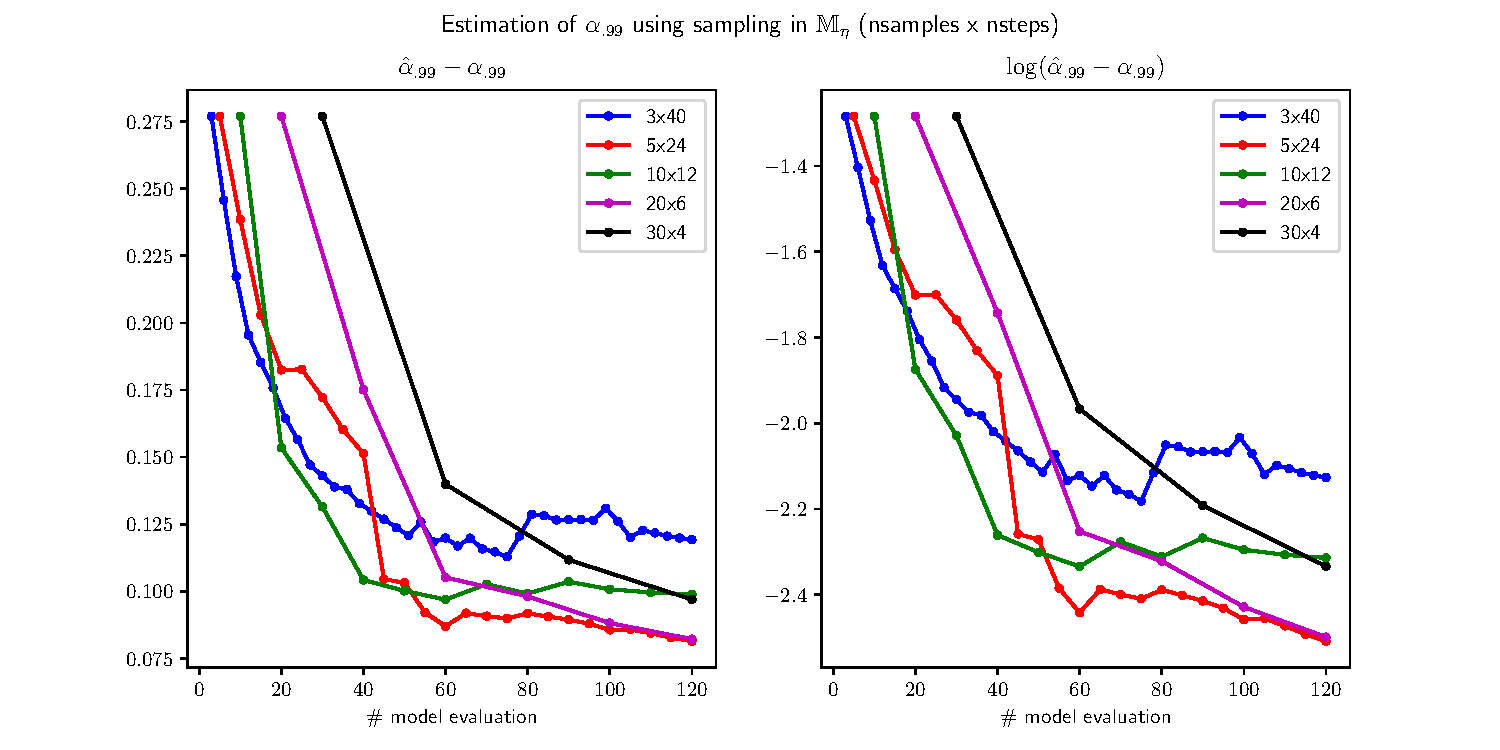
\includegraphics[width=\textwidth]{/home/victor/acadwriting/sampling_estimation_Meta.pdf}
  \caption{\label{fig:label} }
\end{figure}


%%%%%%%%%%%%%%%%%%%%%%%%%%%%%%%%%%%%%%%%%%%%%%%%%%%%%%%
%%%%%%%%%%%%%%%%%%%%%%%%%%%%%%%%%%%%%%%%%%%%%%%%%%%%%%%
%%%%%%%%%%%%%%%%%%%%%%%%%%%%%%%%%%%%%%
%% BIB
%%%%%%%%%%%%%%%%%%%%%%%%%%%%%%%%%%%%%%
\subfileLocal{
	\pagestyle{empty}
	\bibliographystyle{alpha}
	\bibliography{../../bibzotero}
}
\end{document}


%%% Local Variables:
%%% mode: latex
%%% TeX-master: "../../Main_ManuscritThese"
%%% End:
